\documentclass[output=paper,hidelinks]{langscibook}
\ChapterDOI{10.5281/zenodo.10185976}
\title{Morphology in LFG}
\author{Ash Asudeh\affiliation{University of Rochester} and  Daniel Siddiqi\affiliation{Carleton University}}
\abstract{Lexical-Functional Grammar has been consistent over
  the past 4$+$  decades about its conception of syntactic structure
  and the sorts of rules that license it. However, despite being a
  highly lexicalist model of grammar, LFG has not developed a
  similarly consistent model of morphology. LFG has in fact
  assumed a variety of different models of morphology and
  interfaces with distinct \ascare{morphological} modules and theories in
  this time. This is perhaps because LFG early on solved the problem
  of how morphology and syntax can communicate in a common formal
  language — the language of functional descriptions, which can be
  both associated with words and their parts and with syntactic
  elements. We first introduce some important concepts from
  morphological theory. We then  look at some early LFG analyses which
  treated morphology \aterm{incrementally}. Subsequently, we review work on the
  syntax--morphology interface in LFG. We end with a
 discussion of \aterm{realizational} approaches to morphology in LFG.}

\IfFileExists{../localcommands.tex}{
   \addbibresource{../localbibliography.bib}
   \addbibresource{thisvolume.bib}
   % add all extra packages you need to load to this file

\usepackage{tabularx}
\usepackage{multicol}
\usepackage{url}
\urlstyle{same}
%\usepackage{amsmath,amssymb}

% Tight underlining according to https://alexwlchan.net/2017/10/latex-underlines/
\usepackage{contour}
\usepackage[normalem]{ulem}
\renewcommand{\ULdepth}{1.8pt}
\contourlength{0.8pt}
\newcommand{\tightuline}[1]{%
  \uline{\phantom{#1}}%
  \llap{\contour{white}{#1}}}
  
\usepackage{listings}
\lstset{basicstyle=\ttfamily,tabsize=2,breaklines=true}

% \usepackage{langsci-basic}
\usepackage{langsci-optional}
\usepackage[danger]{langsci-lgr}
\usepackage{langsci-gb4e}
%\usepackage{langsci-linguex}
%\usepackage{langsci-forest-setup}
\usepackage[tikz]{langsci-avm} % added tikz flag, 29 July 21
% \usepackage{langsci-textipa}

\usepackage[linguistics,edges]{forest}
\usepackage{tikz-qtree}
\usetikzlibrary{positioning, tikzmark, arrows.meta, calc, matrix, shapes.symbols}
\usetikzlibrary{arrows, arrows.meta, shapes, chains, decorations.text}

%%%%%%%%%%%%%%%%%%%%% Packages for all chapters

% arrows and lines between structures
\usepackage{pst-node}

% lfg attributes and values, lines (relies on pst-node), lexical entries, phrase structure rules
\usepackage{packages/lfg-abbrevs}

% subfigures
\usepackage{subcaption}

% macros for small illustrations in the glossary
\usepackage{./packages/picins}

%%%%%%%%%%%%%%%%%%%%% Packages from contributors

% % Simpler Syntax packages
\usepackage{bm}
\tikzstyle{block} = [rectangle, draw, text width=5em, text centered, minimum height=3em]
\tikzstyle{line} = [draw, thick, -latex']

% Dependency packages
\usepackage{tikz-dependency}
%\usepackage{sdrt}

\usepackage{soul}

\usepackage[notipa]{ot-tableau}

% Historical
\usepackage{stackengine}
\usepackage{bigdelim}

% Morphology
\usepackage{./packages/prooftree}
\usepackage{arydshln}
\usepackage{stmaryrd}

% TAG
\usepackage{pbox}

\usepackage{langsci-branding}

   % %%%%%%%%% lang sci press commands

\newcommand*{\orcid}{}

\makeatletter
\let\thetitle\@title
\let\theauthor\@author
\makeatother

\newcommand{\togglepaper}[1][0]{
   \bibliography{../localbibliography}
   \papernote{\scriptsize\normalfont
     \theauthor.
     \titleTemp.
     To appear in:
     Dalrymple, Mary (ed.).
     Handbook of Lexical Functional Grammar.
     Berlin: Language Science Press. [preliminary page numbering]
   }
   \pagenumbering{roman}
   \setcounter{chapter}{#1}
   \addtocounter{chapter}{-1}
}

\DeclareOldFontCommand{\rm}{\normalfont\rmfamily}{\mathrm}
\DeclareOldFontCommand{\sf}{\normalfont\sffamily}{\mathsf}
\DeclareOldFontCommand{\tt}{\normalfont\ttfamily}{\mathtt}
\DeclareOldFontCommand{\bf}{\normalfont\bfseries}{\mathbf}
\DeclareOldFontCommand{\it}{\normalfont\itshape}{\mathit}
\makeatletter
\DeclareOldFontCommand{\sc}{\normalfont\scshape}{\@nomath\sc}
\makeatother

% Bug fix, 3 April 2021
\SetupAffiliations{output in groups = false,
                   separator between two = {\bigskip\\},
                   separator between multiple = {\bigskip\\},
                   separator between final two = {\bigskip\\}
                   }

% commands for all chapters
\setmathfont{LibertinusMath-Additions.otf}[range="22B8]

% punctuation between a sequence of years in a citation
% OLD: \renewcommand{\compcitedelim}{\multicitedelim}
\renewcommand{\compcitedelim}{\addcomma\space}

% \citegen with no parentheses around year
\providecommand{\citegenalt}[2][]{\citeauthor{#2}'s \citeyear*[#1]{#2}}

% avms with plain font, using langsci-avm package
\avmdefinestyle{plain}{attributes=\normalfont,values=\normalfont,types=\normalfont,extraskip=0.2em}
% avms with attributes and values in small caps, using langsci-avm package
\avmdefinestyle{fstr}{attributes=\scshape,values=\scshape,extraskip=0.2em}
% avms with attributes in small caps, values in plain font (from peter sells)
\avmdefinestyle{fstr-ps}{attributes=\scshape,values=\normalfont,extraskip=0.2em}

% reference to previous or following examples, from Stefan
%(\mex{1}) is like \next, referring to the next example
%(\mex{0}) is like \last, referring to the previous example, etc
\makeatletter
\newcommand{\mex}[1]{\the\numexpr\c@equation+#1\relax}
\makeatother

% do not add xspace before these
\xspaceaddexceptions{1234=|*\}\restrict\,}

% Several chapters use evnup -- this is verbatim from lingmacros.sty
\makeatletter
\def\evnup{\@ifnextchar[{\@evnup}{\@evnup[0pt]}}
\def\@evnup[#1]#2{\setbox1=\hbox{#2}%
\dimen1=\ht1 \advance\dimen1 by -.5\baselineskip%
\advance\dimen1 by -#1%
\leavevmode\lower\dimen1\box1}
\makeatother

% Centered entries in tables.  Requires array package.
\newcolumntype{P}[1]{>{\centering\arraybackslash}p{#1}}

% Reference to multiple figures, requested by Victoria Rosen
\newcommand{\figsref}[2]{Figures~\ref{#1}~and~\ref{#2}}
\newcommand{\figsrefthree}[3]{Figures~\ref{#1},~\ref{#2}~and~\ref{#3}}
\newcommand{\figsreffour}[4]{Figures~\ref{#1},~\ref{#2},~\ref{#3}~and~\ref{#4}}
\newcommand{\figsreffive}[5]{Figures~\ref{#1},~\ref{#2},~\ref{#3},~\ref{#4}~and~\ref{#5}}

% Semitic chapter:
\providecommand{\textchi}{χ}

% Prosody chapter
\makeatletter
\providecommand{\leftleadsto}{%
  \mathrel{\mathpalette\reflect@squig\relax}%
}
\newcommand{\reflect@squig}[2]{%
  \reflectbox{$\m@th#1$$\leadsto$}%
}
\makeatother
\newcommand\myrotaL[1]{\mathrel{\rotatebox[origin=c]{#1}{$\leadsto$}}}
\newcommand\Prosleftarrow{\myrotaL{-135}}
\newcommand\myrotaR[1]{\mathrel{\rotatebox[origin=c]{#1}{$\leftleadsto$}}}
\newcommand\Prosrightarrow{\myrotaR{135}}

% Core Concepts chapter
\newcommand{\anterm}[2]{#1\\#2}
\newcommand{\annode}[2]{#1\\#2}

% HPSG chapter
\newcommand{\HPSGphon}[1]{〈#1〉}
% for defining RSRL relations:
\newcommand{\HPSGsfl}{\enskip\ensuremath{\stackrel{\forall{}}{\Longleftarrow{}}}\enskip}
% AVM commands, valid only inside \avm{}
\avmdefinecommand {phon}[phon] { attributes=\itshape } % define a new \phon command
% Forest Set-up
\forestset
  {notin label above/.style={edge label={node[midway,sloped,above,inner sep=0pt]{\strut$\ni$}}},
    notin label below/.style={edge label={node[midway,sloped,below,inner sep=0pt]{\strut$\ni$}}},
  }

% Dependency chapter
\newcommand{\ua}{\ensuremath{\uparrow}}
\newcommand{\da}{\ensuremath{\downarrow}}
\forestset{
  dg edges/.style={for tree={parent anchor=south, child anchor=north,align=center,base=bottom},
                 where n children=0{tier=word,edge=dotted,calign with current edge}{}
                },
dg transfer/.style={edge path={\noexpand\path[\forestoption{edge}, rounded corners=3pt]
    % the line downwards
    (!u.parent anchor)-- +($(0,-l)-(0,4pt)$)-- +($(12pt,-l)-(0,4pt)$)
    % the horizontal line
    ($(!p.north west)+(0,l)-(0,20pt)$)--($(.north east)+(0,l)-(0,20pt)$)\forestoption{edge label};},!p.edge'={}},
% for Tesniere-style junctions
dg junction/.style={no edge, tikz+={\draw (!p.east)--(!.west) (.east)--(!n.west);}    }
}


% Glossary
\makeatletter % does not work with \newcommand
\def\namedlabel#1#2{\begingroup
   \def\@currentlabel{#2}%
   \phantomsection\label{#1}\endgroup
}
\makeatother


\renewcommand{\textopeno}{ɔ}
\providecommand{\textepsilon}{ɛ}

\renewcommand{\textbari}{ɨ}
\renewcommand{\textbaru}{ʉ}
\newcommand{\acutetextbari}{í̵}
\renewcommand{\textlyoghlig}{ɮ}
\renewcommand{\textdyoghlig}{ʤ}
\renewcommand{\textschwa}{ə}
\renewcommand{\textprimstress}{ˈ}
\newcommand{\texteng}{ŋ}
\renewcommand{\textbeltl}{ɬ}
\newcommand{\textramshorns}{ɤ}

\newbool{bookcompile}
\booltrue{bookcompile}
\newcommand{\bookorchapter}[2]{\ifbool{bookcompile}{#1}{#2}}




\renewcommand{\textsci}{ɪ}
\renewcommand{\textturnscripta}{ɒ}

\renewcommand{\textscripta}{ɑ}
\renewcommand{\textteshlig}{ʧ}
\providecommand{\textupsilon}{υ}
\renewcommand{\textyogh}{ʒ}
\newcommand{\textpolhook}{̨}

\renewcommand{\sectref}[1]{Section~\ref{#1}}

%\KOMAoptions{chapterprefix=true}

\renewcommand{\textturnv}{ʌ}
\renewcommand{\textrevepsilon}{ɜ}
\renewcommand{\textsecstress}{ˌ}
\renewcommand{\textscriptv}{ʋ}
\renewcommand{\textglotstop}{ʔ}
\renewcommand{\textrevglotstop}{ʕ}
%\newcommand{\textcrh}{ħ}
\renewcommand{\textesh}{ʃ}

% label for submitted and published chapters
\newcommand{\submitted}{{\color{red}Final version submitted to Language Science Press.}}
\newcommand{\published}{{\color{red}Final version published by
    Language Science Press, available at \url{https://langsci-press.org/catalog/book/312}.}}

% Treebank definitions
\definecolor{tomato}{rgb}{0.9,0,0}
\definecolor{kelly}{rgb}{0,0.65,0}

% Minimalism chapter
\newcommand\tr[1]{$<$\textcolor{gray}{#1}$>$}
\newcommand\gapline{\lower.1ex\hbox to 1.2em{\bf \ \hrulefill\ }}
\newcommand\cnom{{\llap{[}}Case:Nom{\rlap{]}}}
\newcommand\cacc{{\llap{[}}Case:Acc{\rlap{]}}}
\newcommand\tpres{{\llap{[}}Tns:Pres{\rlap{]}}}
\newcommand\fstackwe{{\llap{[}}Tns:Pres{\rlap{]}}\\{\llap{[}}Pers:1{\rlap{]}}\\{\llap{[}}Num:Pl{\rlap{]}}}
\newcommand\fstackone{{\llap{[}}Tns:Past{\rlap{]}}\\{\llap{[}}Pers:\ {\rlap{]}}\\{\llap{[}}Num:\ {\rlap{]}}}
\newcommand\fstacktwo{{\llap{[}}Pers:3{\rlap{]}}\\{\llap{[}}Num:Pl{\rlap{]}}\\{\llap{[}}Case:\ {\rlap{]}}}
\newcommand\fstackthr{{\llap{[}}Tns:Past{\rlap{]}}\\{\llap{[}}Pers:3{\rlap{]}}\\{\llap{[}}Num:Pl{\rlap{]}}} 
\newcommand\fstackfou{{\llap{[}}Pers:3{\rlap{]}}\\{\llap{[}}Num:Pl{\rlap{]}}\\{\llap{[}}Case:Nom{\rlap{]}}}
\newcommand\fstackonefill{{\llap{[}}Tns:Past{\rlap{]}}\\{\llap{[}}Pers:3{\rlap{]}}\\%
  {\llap{[}}Num:Pl{\rlap{]}}}
\newcommand\fstackoneint%
    {{\llap{[}}{\bf Tns:Past}{\rlap{]}}\\{\llap{[}}Pers:\ {\rlap{]}}\\{\llap{[}}Num:\ {\rlap{]}}}
\newcommand\fstacktwoint%
    {{\llap{[}}{\bf Pers:3}{\rlap{]}}\\{\llap{[}}{\bf Num:Pl}{\rlap{]}}\\{\llap{[}}Case:\ {\rlap{]}}}
\newcommand\fstackthrchk%
    {{\llap{[}}{\bf Tns:Past}{\rlap{]}}\\{\llap{[}}{Pers:3}{\rlap{]}}\\%
      {\llap{[}}Num:Pl{\rlap{]}}} 
\newcommand\fstackfouchk%
    {{\llap{[}}{\bf Pers:3}{\rlap{]}}\\{\llap{[}}{\bf Num:Pl}{\rlap{]}}\\%
      {\llap{[}}Case:Nom{\rlap{]}}}
\newcommand\uinfl{{\llap{[}}Infl:\ \ {\rlap{]}}}
\newcommand\inflpass{{\llap{[}}Infl:Pass{\rlap{]}}}
\newcommand\fepp{{\llap{[}}EPP{\rlap{]}}}
\newcommand\sepp{{\llap{[}}\st{EPP}{\rlap{]}}}
\newcommand\rdash{\rlap{\hbox to 24em{\hfill (dashed lines represent
      information flow)}}}


% Computational chapter
\usepackage{./packages/kaplan}
\renewcommand{\red}{\color{lsLightWine}}

% Sinitic
\newcommand{\FRAME}{\textsc{frame}\xspace}
\newcommand{\arglistit}[1]{{\textlangle}\textit{#1}{\textrangle}}

%WestGermanic
\newcommand{\streep}[1]{\mbox{\rule{1pt}{0pt}\rule[.5ex]{#1}{.5pt}\rule{-1pt}{0pt}\rule{-#1}{0pt}}}

\newcommand{\hspaceThis}[1]{\hphantom{#1}}


\newcommand{\FIG}{\textsc{figure}}
\newcommand{\GR}{\textsc{ground}}

%%%%% Morphology
% Single quote
\newcommand{\asquote}[1]{`{#1}'} % Single quotes
\newcommand{\atrns}[1]{\asquote{#1}} % Translation
\newcommand{\attrns}[1]{(\asquote{#1})} % Translation
\newcommand{\ascare}[1]{\asquote{#1}} % Scare quotes
\newcommand{\aqterm}[1]{\asquote{#1}} % Quoted terms
% Double quote
\newcommand{\adquote}[1]{``{#1}''} % Double quotes
\newcommand{\aquoot}[1]{\adquote{#1}} % Quotes
% Italics
\newcommand{\aword}[1]{\textit{#1}}  % mention of word
\newcommand{\aterm}[1]{\textit{#1}}
% Small caps
\newcommand{\amg}[1]{{\textsc{\MakeLowercase{#1}}}}
\newcommand{\ali}[1]{\MakeLowercase{\textsc{#1}}}
\newcommand{\feat}[1]{{\textsc{#1}}}
\newcommand{\val}[1]{\textsc{#1}}
\newcommand{\pred}[1]{\textsc{#1}}
\newcommand{\predvall}[1]{\textsc{#1}}
% Misc commands
\newcommand{\exrr}[2][]{(\ref{ex:#2}{#1})}
\newcommand{\csn}[3][t]{\begin{tabular}[#1]{@{\strut}c@{\strut}}#2\\#3\end{tabular}}
\newcommand{\sem}[2][]{\ensuremath{\left\llbracket \mbox{#2} \right\rrbracket^{#1}}}
\newcommand{\apf}[2][\ensuremath{\sigma}]{\ensuremath{\langle}#2,#1\ensuremath{\rangle}}
\newcommand{\formula}[2][t]{\ensuremath{\begin{array}[#1]{@{\strut}l@{\strut}}#2%
                                         \end{array}}}
\newcommand{\Down}{$\downarrow$}
\newcommand{\Up}{$\uparrow$}
\newcommand{\updown}{$\uparrow=\downarrow$}
\newcommand{\upsigb}{\mbox{\ensuremath{\uparrow\hspace{-0.35em}_\sigma}}}
\newcommand{\lrfg}{L\textsubscript{R}FG} 
\newcommand{\dmroot}{\ensuremath{\sqrt{\hspace{1em}}}}
\newcommand{\amother}{\mbox{\ensuremath{\hat{\raisebox{-.25ex}{\ensuremath{\ast}}}}}}
\newcommand{\expone}{\ensuremath{\xrightarrow{\nu}}}
\newcommand{\sig}{\mbox{$_\sigma\,$}}
\newcommand{\aset}[1]{\{#1\}}
\newcommand{\linimp}{\mbox{\ensuremath{\,\multimap\,}}}
\newcommand{\fsfunc}{\ensuremath{\Phi}\hspace*{-.15em}}
\newcommand{\cons}[1]{\ensuremath{\mbox{\textbf{\textup{#1}}}}}
\newcommand{\amic}[1][]{\cons{MostInformative$_c$}{#1}}
\newcommand{\amif}[1][]{\cons{MostInformative$_f$}{#1}}
\newcommand{\amis}[1][]{\cons{MostInformative$_s$}{#1}}
\newcommand{\amsp}[1][]{\cons{MostSpecific}{#1}}

%Glue
\newcommand{\glues}{Glue Semantics} % macro for consistency
\newcommand{\glue}{Glue} % macro for consistency
\newcommand{\lfgglue}{LFG$+$Glue} 
\newcommand{\scare}[1]{`{#1}'} % Scare quotes
\newcommand{\word}[1]{\textit{#1}}  % mention of word
\newcommand{\dquote}[1]{``{#1}''} % Double quotes
\newcommand{\high}[1]{\textit{#1}} % highlight (italicize)
\newcommand{\laml}{{L}} 
% Left interpretation double bracket
\newcommand{\Lsem}{\ensuremath{\left\llbracket}} 
% Right interpretation double bracket
\newcommand{\Rsem}{\ensuremath{\right\rrbracket}} 
\newcommand{\nohigh}[1]{{#1}} % nohighlight (regular font)
% Linear implication elimination
\newcommand{\linimpE}{\mbox{\small\ensuremath{\multimap_{\mathcal{E}}}}}
% Linear implication introduction, plain
\newcommand{\linimpI}{\mbox{\small\ensuremath{\multimap_{\mathcal{I}}}}}
% Linear implication introduction, with flag
\newcommand{\linimpIi}[1]{\mbox{\small\ensuremath{\multimap_{{\mathcal{I}},#1}}}}
% Linear universal elimination
\newcommand{\forallE}{\mbox{\small\ensuremath{\forall_{{\mathcal{E}}}}}}
% Tensor elimination
\newcommand{\tensorEij}[2]{\mbox{\small\ensuremath{\otimes_{{\mathcal{E}},#1,#2}}}}
% CG forward slash
\newcommand{\fs}{\ensuremath{/}} 
% s-structure mapping, no space after                                     
\newcommand{\sigb}{\mbox{$_\sigma$}}
% uparrow with s-structure mapping, with small space after  
\newcommand{\upsig}{\mbox{\ensuremath{\uparrow\hspace{-0.35em}_\sigma\,}}}
\newcommand{\fsa}[1]{\textit{#1}}
\newcommand{\sqz}[1]{#1}
% Angled brackets (types, etc.)
\newcommand{\bracket}[1]{\ensuremath{\left\langle\mbox{\textit{#1}}\right\rangle}}
% glue logic string term
\newcommand{\gterm}[1]{\ensuremath{\mbox{\textup{\textit{#1}}}}}
% abstract grammatical formative
\newcommand{\gform}[1]{\ensuremath{\mbox{\textsc{\textup{#1}}}}}
% let
\newcommand{\llet}[3]{\ensuremath{\mbox{\textsf{let}}~{#1}~\mbox{\textsf{be}}~{#2}~\mbox{\textsf{in}}~{#3}}}
% Word-adorned proof steps
\providecommand{\vformula}[2]{%
  \begin{array}[b]{l}
    \mbox{\textbf{\textit{#1}}}\\%[-0.5ex]
    \formula{#2}
  \end{array}
}

%TAG
\newcommand{\fm}[1]{\textsc{#1}}
\newcommand{\struc}[1]{{#1-struc\-ture}}
\newcommand{\func}[1]{\mbox{#1-function}}
\newcommand{\fstruc}{\struc{f}}
\newcommand{\cstruc}{\struc{c}}
\newcommand{\sstruc}{\struc{s}}
\newcommand{\astruc}{\struc{a}}
\newcommand{\nodelabels}[2]{\rlap{\ensuremath{^{#1}_{#2}}}}
\newcommand{\footnode}{\rlap{\ensuremath{^{*}}}}
\newcommand{\nafootnode}{\rlap{\ensuremath{^{*}_{\nalabel}}}}
\newcommand{\nanode}{\rlap{\ensuremath{_{\nalabel}}}}
\newcommand{\AdjConstrText}[1]{\textnormal{\small #1}}
\newcommand{\nalabel}{\AdjConstrText{NA}}

%Case
\newcommand{\MID}{\textsc{mid}{}\xspace}

%font commands added April 2023 for Control and Case chapters
\def\textthorn{þ}
\def\texteth{ð}
\def\textinvscr{ʁ}
\def\textcrh{ħ}
\def\textgamma{ɣ}

% Coordination
\newcommand{\CONJ}{\textsc{conj}{}\xspace}
\newcommand*{\phtm}[1]{\setbox0=\hbox{#1}\hspace{\wd0}}
\newcommand{\ggl}{\hfill(Google)}
\newcommand{\nkjp}{\hfill(NKJP)}

% LDDs
\newcommand{\ubd}{\attr{ubd}\xspace}
% \newcommand{\disattr}[1]{\blue \attr{#1}}  % on topic/focus path
% \newcommand{\proattr}[1]{\green\attr{#1}}  % On Q/Relpro path
\newcommand{\disattr}[1]{\color{lsMidBlue}\attr{#1}}  % on topic/focus path
\newcommand{\proattr}[1]{\color{lsMidGreen}\attr{#1}}  % On Q/Relpro path
\newcommand{\eestring}{\mbox{$e$}\xspace}
\providecommand{\disj}[1]{\{\attr{#1}\}}
\providecommand{\estring}{\mb{\epsilon}}
\providecommand{\termcomp}[1]{\attr{\backslash {#1}}}
\newcommand{\templatecall}[2]{{\small @}(\attr{#1}\ \attr{#2})}
\newcommand{\xlgf}[1]{(\leftarrow\ \attr{#1})} 
\newcommand{\xrgf}[1]{(\rightarrow\ \attr{#1})}
\newcommand{\rval}[2]{\annobox {\xrgf{#1}\teq\attr{#2}}}
\newcommand{\memb}[1]{\annobox {\downarrow\, \in \xugf{#1}}}
\newcommand{\lgf}[1]{\annobox {\xlgf{#1}}}
\newcommand{\rgf}[1]{\annobox {\xrgf{#1}}}
\newcommand{\rvalc}[2]{\annobox {\xrgf{#1}\teqc\attr{#2}}}
\newcommand{\xgfu}[1]{(\attr{#1}\uparrow)}
\newcommand{\gfu}[1]{\annobox {\xgfu{#1}}}
\newcommand{\nmemb}[3]{\annobox {{#1}\, \in \ngf{#2}{#3}}}
\newcommand{\dgf}[1]{\annobox {\xdgf{#1}}}
\newcommand{\predsfraise}[3]{\annobox {\xugf{pred}\teq\semformraise{#1}{#2}{#3}}}
\newcommand{\semformraise}[3]{\annobox {\textrm{`}\hspace{-.05em}\attr{#1}\langle\attr{#2}\rangle{\attr{#3}}\textrm{'}}}
\newcommand{\teqc}{\hspace{-.1667em}=_c\hspace{-.1667em}} 
\newcommand{\lval}[2]{\annobox {\xlgf{#1}\teq\attr{#2}}}
\newcommand{\xgfd}[1]{(\attr{#1}\downarrow)}
\newcommand{\gfd}[1]{\annobox {\xgfd{#1}}}
\newcommand{\gap}{\rule{.75em}{.5pt}\ }
\newcommand{\gapp}{\rule{.75em}{.5pt}$_p$\ }

% Mapping
% Avoid having to write 'argument structure' a million times
\newcommand{\argstruc}{argument structure}
\newcommand{\Argstruc}{Argument structure}
\newcommand{\emptybracks}{\ensuremath{[\;\;]}}
\newcommand{\emptycurlybracks}{\ensuremath{\{\;\;\}}}
% Drawing lines in structures
\newcommand{\strucconnect}[6]{%
\draw[-stealth] (#1) to[out=#5, in=#6] node[pos=#3, above]{#4} (#2);%
}
\newcommand{\strucconnectdashed}[6]{%
\draw[-stealth, dashed] (#1) to[out=#5, in=#6] node[pos=#3, above]{#4} (#2);%
}
% Attributes for s-structures in the style of lfg-abbrevs.sty
\newcommand{\ARGnum}[1]{\textsc{arg}\textsubscript{#1}}
% Drawing mapping lines
\newcommand{\maplink}[2]{%
\begin{tikzpicture}[baseline=(A.base)]
\node(A){#1\strut};
\node[below = 3ex of A](B){\pbox{\textwidth}{#2}};
\draw ([yshift=-1ex]A.base)--(B);
% \draw (A)--(B);
\end{tikzpicture}}
% long line for extra features
\newcommand{\longmaplink}[2]{%
\begin{tikzpicture}[baseline=(A.base)]
\node(A){#1\strut};
\node[below = 3ex of A](B){\pbox{\textwidth}{#2}};
\draw ([yshift=2.5ex]A.base)--(B);
% \draw (A)--(B);
\end{tikzpicture}%
}
% For drawing upward
\newcommand{\maplinkup}[2]{%
\begin{tikzpicture}[baseline=(A.base)]
\node(A){#1};
\node[above = 3ex of A, anchor=base](B){#2};
\draw (A)--(B);
\end{tikzpicture}}
% Above with arrow going down (for argument adding processes)
\newcommand{\argumentadd}[2]{%
\begin{tikzpicture}[baseline=(A.base)]
\node(A){#1};
\node[above = 3ex of A, anchor=base](B){#2};
\draw[latex-] ([yshift=2ex]A.base)--([yshift=-1ex]B.center);
\end{tikzpicture}}
% Going up to the left
\newcommand{\maplinkupleft}[2]{%
\begin{tikzpicture}[baseline=(A.base)]
\node(A){#1};
\node[above left = 3ex of A, anchor=base](B){#2};
\draw (A)--(B);
\end{tikzpicture}}
% Going up to the right
\newcommand{\maplinkupright}[2]{%
\begin{tikzpicture}[baseline=(A.base)]
\node(A){#1};
\node[above right = 3ex of A, anchor=base](B){#2};
\draw (A)--(B);
\end{tikzpicture}}
% Argument fusion
\newenvironment{tikzsentence}{\begin{tikzpicture}[baseline=0pt, 
  anchor=base, outer sep=0pt, ampersand replacement=\&
   ]}{\end{tikzpicture}}
\newcommand{\Subnode}[2]{\subnode[inner sep=1pt]{#1}{#2\strut}}
\newcommand{\connectbelow}[3]{\draw[inner sep=0pt] ([yshift=0.5ex]#1.south) -- ++ (south:#3ex)
  -| ([yshift=0.5ex]#2.south);}
\newcommand{\connectabove}[3]{\draw[inner sep=0pt] ([yshift=0ex]#1.north) -- ++ (north:#3ex)
  -| ([yshift=0ex]#2.north);}
  
\newcommand{\ASNode}[2]{\tikz[remember picture,baseline=(#1.base)] \node [anchor=base] (#1) {#2};}

% Austronesian
\newcommand{\LV}{\textsc{lv}\xspace}
\newcommand{\IV}{\textsc{iv}\xspace}
\newcommand{\DV}{\textsc{dv}\xspace}
\newcommand{\PV}{\textsc{pv}\xspace}
\newcommand{\AV}{\textsc{av}\xspace}
\newcommand{\UV}{\textsc{uv}\xspace}

\apptocmd{\appendix}
         {\bookmarksetup{startatroot}}
         {}
         {%
           \AtEndDocument{\typeout{langscibook Warning:}
                          \typeout{It was not possible to set option 'staratroot'}
                          \typeout{for appendix in the backmatter.}}
         }

   %% hyphenation points for line breaks
%% Normally, automatic hyphenation in LaTeX is very good
%% If a word is mis-hyphenated, add it to this file
%%
%% add information to TeX file before \begin{document} with:
%% %% hyphenation points for line breaks
%% Normally, automatic hyphenation in LaTeX is very good
%% If a word is mis-hyphenated, add it to this file
%%
%% add information to TeX file before \begin{document} with:
%% %% hyphenation points for line breaks
%% Normally, automatic hyphenation in LaTeX is very good
%% If a word is mis-hyphenated, add it to this file
%%
%% add information to TeX file before \begin{document} with:
%% \include{localhyphenation}
\hyphenation{
Aus-tin
Bel-ya-ev
Bres-nan
Chom-sky
Eng-lish
Geo-Gram
INESS
Inkelas
Kaplan
Kok-ko-ni-dis
Lacz-kó
Lam-ping
Lu-ra-ghi
Lund-quist
Mcho-mbo
Meu-rer
Nord-lin-ger
PASSIVE
Pa-no-va
Pol-lard
Pro-sod-ic
Prze-piór-kow-ski
Ram-chand
Sa-mo-ye-dic
Tsu-no-da
WCCFL
Wam-ba-ya
Warl-pi-ri
Wes-coat
Wo-lof
Zae-nen
accord-ing
an-a-phor-ic
ana-phor
christ-church
co-description
co-present
con-figur-ation-al
in-effa-bil-ity
mor-phe-mic
mor-pheme
non-com-po-si-tion-al
pros-o-dy
referanse-grammatikk
rep-re-sent
Schätz-le
term-hood
Kip-ar-sky
Kok-ko-ni
Chi-che-\^wa
au-ton-o-mous
Al-si-na
Ma-tsu-mo-to
}

\hyphenation{
Aus-tin
Bel-ya-ev
Bres-nan
Chom-sky
Eng-lish
Geo-Gram
INESS
Inkelas
Kaplan
Kok-ko-ni-dis
Lacz-kó
Lam-ping
Lu-ra-ghi
Lund-quist
Mcho-mbo
Meu-rer
Nord-lin-ger
PASSIVE
Pa-no-va
Pol-lard
Pro-sod-ic
Prze-piór-kow-ski
Ram-chand
Sa-mo-ye-dic
Tsu-no-da
WCCFL
Wam-ba-ya
Warl-pi-ri
Wes-coat
Wo-lof
Zae-nen
accord-ing
an-a-phor-ic
ana-phor
christ-church
co-description
co-present
con-figur-ation-al
in-effa-bil-ity
mor-phe-mic
mor-pheme
non-com-po-si-tion-al
pros-o-dy
referanse-grammatikk
rep-re-sent
Schätz-le
term-hood
Kip-ar-sky
Kok-ko-ni
Chi-che-\^wa
au-ton-o-mous
Al-si-na
Ma-tsu-mo-to
}

\hyphenation{
Aus-tin
Bel-ya-ev
Bres-nan
Chom-sky
Eng-lish
Geo-Gram
INESS
Inkelas
Kaplan
Kok-ko-ni-dis
Lacz-kó
Lam-ping
Lu-ra-ghi
Lund-quist
Mcho-mbo
Meu-rer
Nord-lin-ger
PASSIVE
Pa-no-va
Pol-lard
Pro-sod-ic
Prze-piór-kow-ski
Ram-chand
Sa-mo-ye-dic
Tsu-no-da
WCCFL
Wam-ba-ya
Warl-pi-ri
Wes-coat
Wo-lof
Zae-nen
accord-ing
an-a-phor-ic
ana-phor
christ-church
co-description
co-present
con-figur-ation-al
in-effa-bil-ity
mor-phe-mic
mor-pheme
non-com-po-si-tion-al
pros-o-dy
referanse-grammatikk
rep-re-sent
Schätz-le
term-hood
Kip-ar-sky
Kok-ko-ni
Chi-che-\^wa
au-ton-o-mous
Al-si-na
Ma-tsu-mo-to
}

   \togglepaper[22]%%chapternumber
}{}

\begin{document}
\maketitle
\label{chap:Morphology}

\section{Introduction}
\label{sec:Morph:introduction}

% XXPeriphrasis?

% XXEmpty paradigm cells?

Lexical-Functional Grammar has been fairly consistent over the past
more than four decades about its conception of syntactic structure and the sorts
of rules that license it. However, despite being a highly lexicalist
model of grammar, LFG has not developed a similarly consistent model
of word-formation.  LFG has in fact assumed a variety of different
models of word-formation and interfaces with distinct
\ascare{morphological} modules and theories in this time. This is
perhaps because LFG early on solved the problem of how morphology and
syntax can communicate in a common formal language --- the language of
\aterm{functional descriptions}, which can be both associated with
words and their parts and with syntactic elements. Together with the
Lexicalist Hypothesis \citep[92]{lapointe80,chomsky1970remarks,BresnanEtAl2016},
this entailed that syntactic terminals are morphologically complete
words, with possibly complex associated f-descriptions, but the theory
did not have to really say anything about the exact mechanism for word
formation or how contributions were made to complex f-descriptions by
specific parts of words.  In addition, LFG has distributed what might
be considered aspects of word-formation to various components besides
a lexicon, including for example prosodic or phonological structures
\citep{DM11,Boegel2015}.
 
In this context, it is perhaps better to start this chapter with a
brief overview of some of the range of variation in morphological theory so
that we can better situate LFG in the landscape of morphological
possibilities (\sectref{sec:Morph:morph-theory}). We then look at 
early LFG analyses which treated morphology incrementally
(\sectref{sec:Morph:incr-morph-lfg}). Then we review work on the
syntax--morphology interface in LFG
(\sectref{sec:Morph:interface}). This sets the stage for a look at 
current approaches to morphology in LFG, which are {realizational}
(\sectref{sec:Morph:real-morph-lfg}). We will not have anything to say
about the interactions of morphology, syntax, and prosody in LFG,
because that is covered by another chapter in this volume,
\citetv{chapters/Prosody}.



\section{Morphological theory and terminology}
\label{sec:Morph:morph-theory}

The landscape of morphological theory is defined by many key \ascare{decision
points} that we summarize here for subsequent use.  These decision
points are pretheoretically distinct from each other, but they have a
tendency to cluster together in ways that will be reflected in
morphological theories interfacing with LFG.  We attempt to be neutral
for each decision point, and also as brief as possible.  We leave the
detailed description of these distinctions to sources like
\citet{hockett54}, \citet{beard95}, and \citet{Stu01}, but also textbooks like
\citet{haspelmath;sims10}, which does an especially good job of
describing these decisions.

\subsection{Morphemes vs.\ words}
\label{sec:Morph:morphemes-vs-words}

The first of these is also the most basic.  What are the
\ascare{atoms} of morphological theory?  What are the inputs to
morphological rules?  What are the elements that morphology
manipulates?  Morphological theories fall into two basic classes:
those that subscribe to the \aterm{morpheme hypothesis} and those that
do not.  The former are typically called \aterm{morpheme-based} theories (or
\aterm{morphemic} theories). The latter are typically called
\aterm{word-based} theories (or \aterm{lexemic} theories).

\begin{sloppypar}
  In morpheme-based models, the inputs to morphological operations are
  idealized as one-to-one pairings of sound and meaning called
  \aterm{morphemes}.  Later mor\-pheme-based models, such as
  Distributed Morphology \citep{hallemarantz}, have redefined
  `morpheme' to mean `abstract morphological feature'.
  In these models, the sound-meaning pairing is better considered a
  \aterm{listeme} \citep{disciullo:word} but is often called a
  \aterm{vocabulary item}.  Historically, a \ascare{word} is the
  morphological domain above morphemes.  In most contemporary models
  of this kind, the \ascare{word} is mostly epiphenomenal or refers to
  an extra-morphological domain (typically prosodic/phonological).  In
  this context, a so-called \ascare{simplex word} is nothing more than
  a domain containing only a single morpheme, while a
  so-called \ascare{complex word} is a domain containing more than one
  morpheme.
\end{sloppypar}

In word-based models \citep{aronoff76}, words are the atoms of the grammar.
Morphological operations have words as their input and words as their
outputs.  In contemporary instantiations of word-based models, the
\aterm{input} and \aterm{output} are not really the appropriate
terms. Rather, \ascare{words} have both abstract representations and
phonological representations. The abstract form of a word is called a
\aterm{lexeme}.\footnote{Word-based and lexeme-based models are not
  strictly the same \citep[7]{aronoff94}. For example, not all word-based
  models assume lexemes, and some lexeme-based models are actually not
  word-based in the strict sense (lexemes are taken to be atoms of morphological descriptions, but words are not). For the purposes of this overview this
  simplification suffices. We thank an anonymous reviewer for helping
  us sharpen this point.}  A lexeme is the basic  representation of a
word (often analogized to a dictionary entry).  A lexeme may be
derived from another lexeme via derivational morphology or compounding
(and thus can be complex) but is never inflected.  The phonological
form of 
a word, which is fully inflected, is called a \aterm{word-form}, which
can be conceptualized as a particular, (grammatically)
context-sensitive, instantiation of a word.  The word-forms of a
lexeme are typically organized into paradigms.

\begin{sloppypar}
  There are many reasons why a theory might choose to assume words or
  morphemes --- more than we could possibly summarize in this space.
  We posit the following as an oversimplified summary. The basic
  tendency observed in the crosslinguistic state of affairs is that
  morphology is affixal and morpheme boundaries are clearly
  identifiable.  This is tautologically true in isolating and
  agglutinative languages, but even fusional languages, which almost
  always have \aterm{portmanteau} (many-to-one) morphemes, tend to
  have clear morpheme boundaries.  On the other hand, divergences from
  this tendency are legion and likely exist in every language.
  \aterm{Templatic} (or root-and-pattern) morphology, such as found in
  Semitic languages, is not easily accounted for as
  affixation. \aterm{Stem allomorphy} and \aterm{suppletion},
  especially in high frequency words, often involves a morphological
  alternation without clear morpheme boundaries.  Furthermore, complex
  words frequently have lexicalized meaning, i.e. non-compositional
  meaning that is more than the sum of the contained meanings.  These
  exceptional data are usually given exceptional explanations, such as
  diachronic ones.  Put simply: the morpheme hypothesis captures the
  basic concatenative cross-linguistic tendency of morphology, but
  lacks synchronic empirical coverage of seemingly exceptional data.
  The word hypothesis is its opposite, capturing all the data, but
  needing to attribute the basic concatenative tendency to something
  else, such as diachronic pressures like grammaticalization.
\end{sloppypar}

%\subsection{Item-and-arrangement vs.\  item-and-process vs.\
%word-and-paradigm}
\subsection{Arrangement vs.\  Process vs.\  Paradigm}
\label{sec:Morph:ia-vs-ip-vs-wp}

The second decision point is the types of rules that operate on the
atoms.  This distinction is originally described by \citet{hockett54}
as the contrast between \aterm{item-and-arrangement} (IA),
\aterm{item-and-process} (IP), and \aterm{word-and-paradigm} (WP)
models.  The names for these models reflect their workings. In an IA
model, morphology is simply the set of morphemes in a word and the
arrangement of those morphemes.  Thus, the arrangement itself (which
is essentially simple concatenation) is the only \ascare{morphological
  process}.  In an IP model, rules (such as \aterm{affixation},
\aterm{reduplication}, \aterm{juxtaposition}, \aterm{suppletion},
etc.) are applied to a \aterm{base} (or \aterm{stem}), which may be
complex or simplex, to generate a new complex form.  IP models are
compatible with both morphemes or words being the \aqterm{base}.
Finally, WP models assume the morphology is the process through which
all the word-forms in a word’s paradigm are inferable from each other
via some mechanism that generates a paradigm.

The reasons for adopting any of these three are similar to the reasons
in \sectref{sec:Morph:morphemes-vs-words}.  IA models have two
strengths.  Firstly, they capture the basic cross-linguistic generalization:
the vast majority of morphology can be explained with simple
concatenation.  Secondly, many practitioners of IA models
find such a simple operation to have an elegance and restriction that
are laudable metatheoretical goals.  Because of this, IA would be
preferred by those theorists for whom such theoretical elegance is a
high-ranking concern.  Again, we find that such practitioners are
satisfied that putatively non-concatenative processes have
potential diachronic explanations.

There are familiar reasons to assume IP models, which again, as in
\sectref{sec:Morph:morphemes-vs-words} appear to be the opposing reasons.
Chief among them is that IA models under-describe the data.  IA models
end up accounting for everything with affixation, including apparently
non-affixal morphology like \aterm{functional shift},
\aterm{back-formation}, \aterm{stem allomorphy}, \aterm{suppletion},
\aterm{stress shift}, \aterm{truncation}, and \aterm{reduplication}.
Affixal explanations for these phenomena tend to be fairly stipulative
and lead to a proliferation of null morphemes that condition these
changes (which are themselves a violation of theoretical parsimony,
despite this concern being a primary motivation of such approaches).
IP practitioners point out that there is also a ready-made
counter-explanation from diachrony for the prevalence of
concatenation: the chief source of morphology is grammaticalization,
which (ultimately) leads to affixes.  Furthermore, although rule-based
morphological models are undoubtedly much more powerful than IA
models, that power comes with significant empirical coverage, which is
arguably worth the trade-off.  In many varieties of both WP and IP
models, in the idealized case, any two word-forms can be mutually
predictive.  This allows rules to apply \ascare{backwards}, capturing
phenomena such as \aterm{backformation} or \aterm{cross-formation}
\citep[see, e.g.,][]{Becker1993}.  These types of morphological
alternations are difficult to capture in an IA model. 

The appeal of WP models over the other two is the ability to make
reference to the paradigm as an abstract entity.  In the domain of
inflection, many generalizations, especially \aterm{morphomic} ones,
can be captured by referring to the paradigm itself. A
\aterm{morphome}, as described in \citet{aronoff94} and
\citet{luis;bermudez16-book}, among others, is a purely morphological
pattern. The existences of morphomes is controversial \citep[a debate
captured well in][]{luis;bermudez16-book}. The most salient of
proposed morphomes in this debate are root allomorphy patterns like
the \ascare{L pattern} and the \ascare{N pattern}
\citep[see][]{maiden18}, which
are literally described as patterns in
a paradigm (e.g., cells arranged in an L or an N). Thus WP models are
uniquely well-situated to account for these. On the other hand,
arrangement accounts usually deny the existence of morphomes as
paradigm effects and instead account for them via some other mechanism
\citep[see][]{trommer16}.

    Similarly, patterns of syncretism lend themselves to
    paradigmatic explanations. Paradigmatic explanations are
    especially well suited to highly fusional languages as are common
    in Indo-European.  They also lend themselves easily to complex
    agreement patterns that are cross-linguistically ubiquitous.
    Furthermore, because a paradigm cell can contain multiple forms or
    even no forms, WP models allow explanations for both
    \aterm{optionality} and \aterm{defectiveness}/\aterm{ineffability}.
    The tradeoff here is paradoxical: on the one hand, paradigmatic
    models tend to have little to say about derivation\footnote{There
      are some notable exceptions, though, such as \textcite{Booij2010}
      and \citet{spencer13}.}  and compounding, so they under-describe
    the data; on the other hand, paradigms are much more powerful than
    needed for most of the world’s languages, so in another respect,
    they over-describe the data.\footnote{Word and Paradigm models
      encompass more than just what is described here, including
      adaptive discriminative models such as \citet{blevins;ea16}, but
      these have not yet been meaningfully interfaced with LFG, so we
      set them aside here.}
  
% \subsection{What even \emph{is} the lexicon?}
\subsection{What is the lexicon?}\largerpage[2]

The third decision point is the nature of the word-storage component
of the grammar.  For example: Is the lexicon a productive component of
the grammar or simply a passive list of memorized forms?  While the
terminology here is far from consistent in the literature, for the
purposes of this chapter we will use \aterm{lexicon} to denote a generative/productive
component of the grammar responsible for word-formation.  We will use
\aterm{vocabulary} for a passive component which is simply a list of memorized
items.  There is nothing inherently contradictory about a model having
both a lexicon and a vocabulary.  It just happens that most models
with a productive component typically assume that that component is
also the one responsible for word-storage.  Indeed, this dual role is
central to many models of \aterm{blocking}, such as the original one developed
by \citet{aronoff76}.  On the other hand, \citet{disciullo:word}
argue for both a lexicon and a vocabulary (without using those
terms). 
% \citep[for discussion and
% references, see][102--105]{haspelmath;sims10} Booij 1996

There are some downstream effects of the decision to have a component
dedicated to word-formation.  If it is assumed that the lexicon is
productive, a decision must be made on how much it is responsible for.
The \aterm{Single Component Hypothesis} claims that all three
distinct types of morphology (derivation, inflection, and compounding)
are handled by the same generative component.  On the other hand, the
\aterm{Split Morphology Hypothesis} claims that derivation
and inflection are handled by separate components.  Thus, it is not
uncommon to have two distinct word-formation components, one for
derivation and one for inflection, depending on a particular
model's definition of \aterm{lexeme}. This is made explicit in the WP
model of \citet{anderson82-wm,anderson92}, where the paradigms are
only responsible for inflection.\footnote{Split morphology theories are
properly ambivalent about the place of compounding; we do not address
compounding in this chapter.}

Provided you assume that morphology is not its own domain, there seem
to be two obvious non-morphological components involved in ordering 
morphological elements.  One of these is prosody/phonology, as seen in
models such as Optimality Theory \citep{PrinceSmolensky2004}.  The
other, more common, account for ordering morphological elements outside of
a lexicon is the syntactic component.  The \aterm{Morphosyntax
  Hypothesis} --- this is not its common name but will suit our
purposes --- assumes that all of morphology and syntax are handled by
the same component of the grammar. This entails the strong claim that
autonomous morphological phenomena do not exist, and are instead
attributable to the morphological interfaces with phonology and
syntax. The \aterm{Weak Lexicalist Hypothesis} separates derivation
from inflection: Derivation is handled by a lexicon while inflection
is part of the syntactic structure.  By contrast, the \aterm{Strong
  Lexicalist Hypothesis} assumes that all of
word-formation is Lexical/non-syntactic.

We won’t get into the reasons why a syntax model might adopt
variations on the Lexicalist Hypothesis.  We leave that to elsewhere
in this handbook.  From the point of view of morphological theory,
there are distinct reasons to consider breaking the class of things
called \aqterm{word-formation} into distinct components.  Data on morphological
structure suggests compounding
and derivation are of a kind that is distinct from inflection.   In the
domain of derivation and compounding, fully productive morpheme
ordering overwhelmingly generalizes as \aterm{headed hierarchical structure}
(the type of structure usually represented by trees in syntactic theory).  In inflection, on
the other hand, to the extent that morpheme boundaries are even
identifiable, they tend to be arranged in ordered flat
  structure (i.e., a \aterm{list}). Constituency tests that show hierarchical structure tend to fail,
despite strict ordering. Alternatively, when boundaries are less
identifiable, the morphology appears to be arranged \aterm{paradigmatically}.
This difference is mostly captured by the distinction between an
agglutinative and a fusional inflectional system.  A key reason for
treating inflection as different from other kinds of morphology is
precisely because of the apparent 
structural distinction between a linear structure (inflection) and a
hierarchical structure (derivation). Conversely, while inflection is overwhelmingly productive
and expresses compositional meaning, derivation and compounding have a
much greater (but still small) likelihood of having non-compositional
meaning and being less than fully productive.   This is yet another
reason to partition morphology into distinct classes. 

Finally, and perhaps most importantly, to the extent that we can today
justify that derivation is a distinct empirical category from
inflection, following \citet{anderson82-wm}, the chief generally
observed distinction (outside of the hierarchical/linear/paradigmatic
ones above) is that inflection is relevant to the syntax.  Inflection
comes in two varieties.  The first empirical category is those
inflections that express grammatical configurations \citep[\aterm{contextual inflection;}][]{booij96}.  For example,
case and subject/object agreement on verbs express the relationship
between verbs and their dependents.  Similarly, nominal concord
expresses the relationship between nouns and their dependents.
Importantly, languages appear to have the option of expressing these
relationships either via morphology or through a fixed word order (or
both).  The other empirical category of inflection is those
morphological reflexes of so-called \aqterm{morphosyntactic} or \aqterm{morphosemantic}
categories \citep[\aterm{inherent inflection;}][]{booij96}.  These are such properties as tense, aspect, voice, mood,
number, definiteness, etc.  Again, languages appear to have the choice
of expressing these properties morphologically or syntactically
(through separate categories such as auxiliaries, clitics, prepositions, etc).

Given these differences, it makes sense to split a \aterm{lexicon} into two
pieces: one that handles so-called \aterm{lexeme-formation} and
another that handles inflection (but see \citealt{booij96} for
counter-arguments).  These two components can then have fundamentally
different types of processes and can have different relationships with
the syntactic component.  And indeed, this division of labor is common
in Word-and-Paradigm models today. For a review of the history and
state-of-the-art of WP models, see \citet{blevins18}.

\begin{sloppypar}
  Since syntax is also naturally represented, at least in part, by
  headed hierarchical structures, the parsimonious approach to grammar
  is to identify the extent to which all such structure can be done
  with the same component --- in other words, to assume a single
  component that generates headed hierarchical structure, whether the
  structure represents \ascare{syntax} or \ascare{morphology}.
  Compounding and derivation can similarly easily be accommodated to a
  component that generates headed hierarchical structure, especially if
  we restrict the model to only the most productive processes and we
  are willing to assume that non-compositional morphological meaning
  is fundamentally the same as non-compositional idiomatic syntactic
  constructions.  We would have to then be willing to postulate
  vacuous hierarchical structure in inflection, but this postulation is
  arguably worth the trade-off for overall parsimony. The call of
  parsimony is heightened by the definitional interdependence of
  syntax and inflection.  In fact, an Item-and-Arrangement model has
  already made certain empirical sacrifices for parsimony and
  restriction goals.  It seems that no further sacrifices are needed
  to assume a single morphosyntactic component.  The gain in parsimony
  is even further support for Item-and-Arrangement from this point of
  view, so it is not surprising that most models today that assume an
  Item-and-Arrangement model reject the Lexicalist Hypothesis and
  adopt a passive \aterm{vocabulary}.  But deciding to approach morphology by
  reducing it to syntactic (and/or phonological) operations is not
  restricted to Item-and-Arrangement approaches.  Similarly,
  \aterm{construction-based} approaches to morphology
  \citep{Booij2010,masini;audring18} generally assume that the
  \aterm{construction} is both a morphological and syntactic
  mechanism. This property of having a shared mechanism is often
  summarized as \ascare{X all the way down}, where X is
  \aterm{constructions} in construction-based approaches,
  \aterm{syntax} in standard Distributed Morphology, and
  \aterm{constraints} in Lexical-Realizational Functional Grammar.
\end{sloppypar}

Approaching morphology via a single morphosyntactic component has
significant empirical justifications as well.  There are several
commonplace phenomena that blur the lines between word and phrase,
suggesting that distinction is more one of convenience than a
justifiable categorical contrast.  Such phenomena include for example:
clitics, phrasal affixes, phrasal compounds, valence changing devices,
separable prefixes (of the Germanic variety; e.g., \citealt{booij02}), object incorporation (of
the Mohawk variety; e.g., \citealt{Baker1988}).  Because these phenomena appear to be both syntactic
and morphological, it is appealing to these practitioners to find
unitary explanations, which ultimately rest on not positing a syntax/morphology distinction. 

\subsection{Lexical vs.\ inferential}
\label{sec:Morph:lexic-vs-infer}

While not strictly distinct from our classification above, it is worth
taking a moment to describe a distinction that is common in the literature,
especially within models that interface with LFG.  \citegen{Stu01} 
typology of morphological theories of inflection includes a
distinction between two types of theory:  \aterm{Lexical} and \aterm{Inferential}.  In
a lexical model, the lexicon (or vocabulary) stores 
associations of inflectional properties and phonological properties. A
complex word is an ordered set of these associations.
Conversely, in an inferential model, the systematic associations are
between a lexeme and its word-forms.  Word-forms are inferred from their
stems by rules (not restricted to concatenation) that
associate aspects of form with aspects of grammatical content. In sum,
lexical models are concerned with listed lexical objects (words or
morphemes), whereas inferential ones are concerned with rules. 

In the typology that we are describing here, these distinctions are
not basic.  Instead, they are composites of the distinctions above.
While it may not be the case that \citet{Stu01} intends \aquoot{lexical} to
comprise these four properties, the examples of \aterm{lexical} models that 
\citet{Stu01} lists all share in common that they are \aterm{morpheme-based},
\aterm{Item-and-Arrangement}, and \aterm{morphosyntactic} with a passive \aterm{vocabulary}.  In
contrast, an \aterm{inferential} model is \aterm{word-based}, and
assumes \aterm{Strong Lexicalism}
(at least for inflection, which is what \citealt{Stu01} is concerned with).


\subsection{Incremental vs.\ realizational}
\label{sec:Morph:incr-vs-real}


The final distinction that we describe here concerns the relationship
between information and morphology.  In an incremental model,
morphology is \aterm{information-adding}.  That is,
a word gains grammatical complexity (i.e., morphosyntactic properties)
at the same time, or as a function of, gaining complex morphology.
For example, on this conception, adding the plural morpheme to the word is what makes it
plural.  In opposition to this stand \aterm{realizational} models.  In
a realizational model, morphology is \aterm{information-expressing}.
Some aspect of grammar that is external to the morphology supplies a
set of morphosyntactic properties (which may or may not include a
\aterm{root}).  What we conceptualize as morphology then expresses
that set of morphosyntactic features. Depending on other choices made,
this expression might be a passive mapping to phonology or the
application of a realizational rule.  In these models, morphology
provides the \aterm{exponence} of morphological properties (the
\aterm{exponenda}).

This distinction is not so much an active distinction today since most
contemporary morphologists assume \emph{some} variety of realizational
morphology. This can be achieved via paradigms (Paradigm Function
Morphology; \citealt{Stu01,stump16,spencer13}), morpheme-insertion
(Distributed Morphology; \citealt{hallemarantz}), or constructions
(Construction Morphology; \citealt{Booij2010,masini;audring18};
Optimal Construction Morphology;
\citealt{inkelas;ea06,caballero;inkelas13,inkelas16}). The simple
reason for this is that morphology, especially inflection, both under-
and overdetermines its featural content.

The underdetermination part
has always been well-known.  For example, a fundamental property of
inflection and primary explanandum of morphological theory is the fact
that the morphosyntactic features overtly expressed by an inflected
form are often a subset of those properties that are associated with
the word.  For example, it is common for gender to be unexpressed in
combination with participant persons (1\textsuperscript{st} and
2\textsuperscript{nd}). Similarly, it is also common for person
features to be unexpressed in combination with past tense or plural
number \citep[see, for example,][]{bjorkman;ea21}. 

Interestingly, the reverse is true as well, which demonstrates 
the case of overdetermination.  Morphosyntactic properties are often
expressed \emph{multiply} without additive meanings; this is usually
called \aterm{multiple exponence}.  For example, \aword{children} is
not \ascare{multiply plural} despite having three distinct reflexes of
plural (vowel change, historic \aword{-r} plural, historic \aword{-en}
plural). What is noteworthy here is that the multiple expression of
plurality is \emph{grammatical}. One wouldn't expect this of an
iterated plural function, which is what multiple applications of a
plural morpheme might lead one to expect \citep[see, for example,][]{harris16}.



\section{Incremental morphology and LFG}
\label{sec:Morph:incr-morph-lfg}

\subsection{Phrase structure rules as word-formation rules}
\label{sec:Morph:psr-wfr}

An obvious approach to concatenative morphology is to capture
morphological well-formedness using similar (annotated) phrase
structure rules to the ones that license c-structures
\citep{selkirk82}. The difference is that the morphological ones use
morphological categories. However, standard LFG assumes \aterm{Strong
  Lexicalism}, so it is important to note that this is happening in
different combinatorial components of the grammar --- morphology
versus syntax. Pedagogical presentations, such as
\citet{BresnanEtAl2016}, out of necessity simplify representations in
such a way that this important distinction is masked. In the problem
set on West Greenlandic \citep[364--369]{BresnanEtAl2016}, we find the
example in \exrr{green-ex} below, analyzed with the assistance of the
morphological rule in \exrr{green-rule}, and the sketch of an analysis
for \exrr{green-ex} in \exrr{green-sol}.\footnote{We have left the
  morphological glosses off the free English translation in
  \exrr{green-sol}, which is not present in
  \citet[446]{BresnanEtAl2016}; this is just a rough approximation of
  the glossing in \exrr{green-ex}. We have also elided some
  annotations from the original.}
%
\ea \label{ex:green-ex} West Greenlandic\\
\gll
    Angisuu-mik qimmeq-arpoq.\\
    big-\amg{ins} dog-have.\amg{ind}.3.\amg{sg}\\
\glt `He has a big dog.'
\ex \label{ex:green-rule}
  \phraserule{V}{\csn{N\textsubscript{stem}}{(\UP\OBL) $=$
      \Down} {\ \ } \csn{V\textsubscript{suff}}{\updown}}
\z
%
Note that this rule looks just like a c-structure rule, except with a
c-structure category on the lefthand side of the rule and
morphological categories on the righthand side. In other words, it is the
\emph{outputs} of these morphological rules that form the
\emph{inputs} to the c-structure rules.
%
\ea \label{ex:green-sol}
  \begin{forest} 
    [S
      [\csn{(\UP\OBL) $=$ \Down}{NP}
        [\csn{(\UP\ADJ) $=$ \Down\\
                                          \vdots}{N}
          [{\aword{angisuumik}\\\atrns{big}}]
        ]
      ]
      [\csn{\updown}{V}
        [\csn{(\UP\OBL) $=$ \Down}{N\textsubscript{stem}}
          [\aword{qimmeq}\\
                            \atrns{dog}
          ]
        ]
        [\csn{\updown}{V\textsubscript{suff}}
          [\aword{arpoq}\\\atrns{has}]
        ]
      ]
    ]
  \end{forest}
\z
However, notice that the node labelled V in this tree is actually
licensed by the \emph{morphological} rule in \exrr{green-rule}. In
another sense, this very same V is also licensed by the c-structure
rule for S, which is easily inferable from \exrr{green-sol}.  

However, if morphology and syntax are distinct grammatical modules,
per Strong Lexicalism, then it can't actually be a single rule set
that captures both aspects of V, as implied by \exrr{green-sol}, even
if the mechanisms involved are the very same for both syntax and
morphology (annotated phrase structure rules) in this incremental
approach to LFG morphology. Thus, a more transparent way to represent
\exrr{green-sol} may be something like the following \citep[based on][285]{Ishikawa1985}: 
%
\eabox{ \attop{
  \begin{forest} 
    [S
    [\csn{(\UP\OBL) $=$ \Down}{NP}
    [\csn{(\UP\ADJ) $=$ \Down\\
                                      \vdots}{N} [\aword{angisuumik}\\
                                                                        \atrns{big}]]]
    [\csn{\updown}{V\\
                      \textbardbl\\[-1.25ex]
                                    \rule{3em}{.75pt}\\
                                                        \textbardbl\\
                                                                      V}
    [\csn{(\UP\OBL) $=$ \Down}{N\textsubscript{stem}} [\aword{qimmeq}\\
                                                                                \atrns{dog}]]
    [\csn{\updown}{V\textsubscript{suff}} [\aword{arpoq}\\
                                                          \atrns{has}]]
    ]]
  \end{forest}
}
}
%
The horizontal line represents the syntax/morphology \ascare{boundary}
and we see that V has a foot on each side. This representation is
arguably more transparent about the full set of theoretical claims
behind \exrr{green-sol}. But it also highlights that the licensing
mechanisms for c-structure and morphology are redundant in this
sort of incremental morphology for LFG.

It is important to realize, though, that in early LFG, incremental
morphology through phrase structure rules was not merely a pedagogical
simplification. There were proposals in early LFG research on morphologically rich
languages that involved phrase-structural incremental morphology, such
as \citet{baker83}, \citet[ch.\,3]{Ishikawa1985}\footnote{See \citet[396]{BresnanEtAl2016} for
a simplified presentation of some of \citeauthor{Ishikawa1985}'s
proposals.} and \citet{nordlinger97,nordlinger1998constructive}. For example,
\citet[107]{nordlinger97} proposes the following morphological rule
for case affixation in various dependent-marking languages of
Australia (including, e.g.,  Kayardild, Martuthunira, Thalanyji, Wambaya):
%
\ea
\phraserule{N}{\csn{N}{\updown} {\ \ } \csn{Aff}{\updown}}
\z
%
\citeauthor{nordlinger97} subsequently revised this incremental
analysis in favour of a realizational approach
\citep{sadler-nordlinger2004,SadlNord2006}, which will be
discussed further in \sectref{sec:Morph:lfg-pfm}.  

In sum, the early incremental approach to
morphology that was commonly assumed by LFG was a straightforward,
even traditional, \aterm{morpheme-based}, \aterm{item-and-arrangement}
approach.

% The
% morphological component, as is standardly assumed in LFG, was
% critically distinct from the syntax, but as shown in \exrr{}, this
% followed from the theory of syntax rather than the theory of
% morphology. XX

\subsection{Finite-state morphology}
   
\begin{sloppypar}
  Another question that arises with incremental phrase-structural
  morphology is one of computational complexity/power. One way of
  expressing the intuition that morphology is generally concatenative
  is to observe that regular languages/finite state automata, which
  are the Type~3 grammars in the Chomsky Hierarchy
  \citep[part~E]{chomsky1957syntactic,chomsky65-hier,partee-etal1990}, are
  computationally sufficient for generating concatenative
  morphology. One can make an even stronger claim, which is that  
  almost all of morphology requires no more than finite-state power,
  except for total reduplication
  \citep[25,~53--60]{beesleykarttunen03,roark;sproat07}, which is
  beyond finite-state power, since it requires exactly matching
  a preceding string of potentially unlimited length.\footnote{Note
    that \citet{beesleykarttunen03} build their system around the
    operation of \aterm{concatenation}, whereas \citet{roark;sproat07}
    argue that the operation of \aterm{composition} is more general
    and is to be preferred. Among other considerations,
    \aterm{composition} gives a more natural finite-state solution to
    templatic (root-and-pattern) morphology
    \citep[41--44]{kiraz01,roark;sproat07}.}
\end{sloppypar}

\begin{sloppypar}
  Let's now turn back to the particular kinds of proposals for
  phrase-structural morphology that we saw in
  \sectref{sec:Morph:psr-wfr}. The computational power of
  phrase-structural morphology is at least context-free, which is more
  powerful than required and corresponds to a higher level in the
  hierarchy.  In other words, representing concatenative morphology in
  a phrase structure format gives the morphological component more
  potential power than seems justified by linguistic data.
  % Having said this, it's also important to bear in mind
  % that not \emph{all} patterns that are considered in whole or at
  % least in part morphological are concatenative (cf. total
  % reduplication).
  Moreover, once we add f-structure annotations to morphological
  phrase structure rules, we are potentially in the yet more powerful
  class of mildly context-sensitive languages \citep{joshi-etal1991},
  since we would have the full power of LFG. This seems too powerful.
\end{sloppypar}


    For example, if morphology were mildly context-sensitive, we might
    expect to see \emph{morphological} long-distance dependencies or
    cross-serial dependencies, but we are not aware of any
    morphological phenomena that straightforwardly demand such
    analyses. It might seem that phenomena such
      as circumfixion or vowel harmony are  candidates for
      morphological long-distance dependencies, but these can in fact be handled by
      finite-state means \citep{beesleykarttunen03}. Some agreement
      phenomena, like the Ojibwe \feat{person} discontinuity
      in \exrr{ojibwe-see} below, might similarly seem long-distance, but
      are in fact clause-bounded, so we expect that finite-state morphology (FSM) could handle
      them. We are aware of so-called \ascare{long-distance agreement}
      \citep{butt93-bls,bhatt05-lda}, but we are not aware of any such case for which there is
      no viable non-long-distance solution. Lastly, it
      might seem that templatic morphology shows a morphological
      need for an indexed language (mildly context-sensitive) to line
      up consonants and vowels properly. However, it has been shown
      that a composition-based finite-state approach can indeed handle
      templatic morphology \citep{kiraz01,roark;sproat07}.
        
      It should be noted that actual computational work on LFG, in the
      context of the Parallel Grammars (ParGram) project
      (\citealt{ButtEtAl1999}; \citetv{chapters/ImplementationsApplications}), uses finite-state
      morphology, rather than incremental phrase-structure
      morphology. Indonesian is among the languages in the ParGram
      project and does have productive total reduplication. The
      ParGram Indonesian grammar only allows for reduplication of
      words already in the dictionary/lexicon. This means that the FSM
      can extract the morphological feature encoded by the
      reduplication (because there is a finite vocabulary). However,
      on encountering a word for the first time, such a system cannot
      recognize the reduplication and so cannot extract the morphological
      feature encoded.\footnote{We thank Ron Kaplan (p.c.) for
        discussion of this point. Any remaining errors are our own.}
      Thus, the full productivity of Indonesian reduplication is not
      modelled in the ParGram grammar.
  
  \begin{sloppypar}
    In sum, the FSM approach is a restrictive approach that also
    yields broad coverage of morphological phenomena; for example, see
    the many case studies in \citet{roark;sproat07}. The
    restrictiveness of the FSM approach makes it very attractive,
    even more so when coupled with the fact that FSM approaches
    have revolutionized applications that require morphological
    analysis, such as spell-checkers, part-of-speech taggers, and
    speech recognition and production systems 
    \citep{KaplanKay1994,beesleykarttunen03,roark;sproat07}. Nevertheless,
    this does not mean that we should conflate theories with their
    formal or computational bases. Using an analogy from syntax, the
    mildly context-sensitive formalisms of Lexicalized Tree-Adjoining
    Grammar, Categorial Grammar, and LFG form a computational
    equivalence class but nevertheless underpin distinct theories. As
    \citet{roark;sproat07} themselves emphasize, theoretical
    distinctions may matter even if the options are computationally
    equivalent. For example, they consider Tagalog \aword{-um-}
    infixation, as in \aword{tawag} \attrns{call} versus
    \aword{tumawag} \attrns{call (perfective)}. They note that it is
    computationally ``immaterial'' from an FSM perspective whether we
    conceive of the infix as attaching to \aword{t-} or to
    \aword{-awag} \citep[30--31]{roark;sproat07}. However, from a
    theoretical perspective, these two solutions are clearly not
    equivalent. In particular, Tagalog \aword{um} is an infix in
    consonant-initial words (with some exceptions, where it cannot
    appear at all), but is a \emph{prefix} in vowel-initial words, such
    as \aword{abot}, which becomes \aword{umabot} \attrns{reach
      for (perfective)} \citep[204]{orgun;sprouse99}. On theoretical grounds, it
    therefore seems preferable to think of \aword{um} as attaching to
    the element to its right, as \citet{McCarthyPrince1993} and
    \citet{orgun;sprouse99} conclude, but to FSM the two options
    (dependency on the preceding or following element) are equivalent
    and the distinction immaterial.
    % For example, in the related Philippine language,
    % Bontoc, \aword{-um-} is likewise an infix in consonant-initial
    % words, such as kum\'{}\v{a}w\v{\i}sat \attrns{I am getting
    %   better}, but is a prefix in vowel-initial words, such as
    % umantj\'{}\v{o}ak \attrns{I am getting taller}
    % \citep[39]{roark;sproat07}. It therefore seems preferable to think
    % of \aword{um} as attaching to the element to its right, rather
    % than to its left.
  \end{sloppypar}
  
\subsection{Lexical rules}
\label{sec:Morph:lexical-rules}

Throughout the early history of LFG, theorists made crucial use of
\aterm{lexical rules}, such as found in \citet{bresnan1982the-passive}.  These
lexical rules were almost always employed to capture argument
structure alternations, like passivization. Another way to think
about the effect of lexical rules is that they concern the remapping
of grammatical functions.  These rules frequently had morphological
reflexes in addition to their argument-structure-changing properties,
but they also frequently did not \citep[see the example lexical rules
for gerundives in][316--317]{BresnanEtAl2016}. In
fairness, these rules were not normally postulated from the point of
view of morphological theory, so the emphasis was not on their
morphological reflexes or how to use them to capture morphological
generalizations. Moreover, lexical rules were not systematically
codified into a model that we could discuss explicitly here.


Nevertheless, it was clear that these rules
are explicitly non-syntactic.  For example, in \citeauthor{falk2001lexical}’s
textbook they are described thus \citep[93]{falk2001lexical}:
\begin{quote}
[A] lexical rule of this kind is not monotonic: it takes existing
information and changes it. This is ruled out in principle in the
syntax on grounds of processing: syntactic information cannot be
changed. But a lexical rule is not a syntactic rule. Lexical rules do
not represent on-line processing, but rather regularities relating
stored lexical items. When a lexical rule is applied productively, the
result is stored as a new lexical item. For this reason, the usual LFG
constraint against changing information is inapplicable here. 
\end{quote}
%
\citeauthor{falk2001lexical}'s pedagogical point is revealing of an important
foundational tenet of LFG: syntax is monotonic, so no non-monotonicity
can be syntactic. It therefore follows that argument alternations are
non-syntactic, since they are non-monotonic. In other words, allowing the
lexical rules to behave non-monotonically shields the syntax. 

On the other hand, \citet{baker85} explicitly considers lexical rules
from the point of view of morphological theory, arguing precisely that
because GF-rules (argument structure rules) and word-formation rules
align on the same element in LFG \citep[i.e., the lexical rule as
developed in][]{bresnan1982the-passive}, LFG was especially well equipped to capture
the \aquoot{lexicalist approach} to the Mirror Principle
\citep[409]{baker85}.  To the extent that these lexical rules were
codifiable in the categories we have laid out, these rules often
generated affixation as in the types described by \citet{baker85}, but
most frequently required the power and mechanisms of an 
\aterm{Item-and-Process} approach to morphology, especially because they were
often expressed with non-concatenative (frequently null) morphology
and were explicitly both information-adding and information-destroying,
the latter of which cannot be done with concatenation alone.

% The reason we place lexical rules in the category of incremental
% morphology is because they are in effect a non-branching phrase
% structure rule that maps one lexical entry to another 

% Lexical rule approaches:
% \begin{itemize}[leftmargin=*]
% \item Refs: \citet{buttking2005}, \citet{Toivonen02},
%   \citet{falk01}
% \item Things lexical rules have been proposed for: argument structure
%   changes (which may or may not have morphological expression)
%   $\Rightarrow$ LMT $\Rightarrow$ Glue approaches 
% \end{itemize}



% \subsection{Realizational morphology in LFG}

\section{The syntax--morphology interface}
\label{sec:Morph:interface}

Some work on morphologically conditioned syntactic order (e.g.,
restrictions on verbal sequences, as found in English \ascare{affix
  hopping}; \citealt{chomsky1957syntactic}) has proposed a structure called m(orphological)-structure
to shield f-structure from features that are morphological in nature
\citep{buttetal96,FrankZaenen2004}. This unfortunately gives the
impression that m-structure is the morphological component of LFG, but
this is not really the case, as we'll see in
\sectref{sec:Morph:m-structure}. First, though, we turn to a general
framework for the interface between an LFG syntax and a realizational
morphology \citep{dalrymple15}. This better sets the context for the
discussion of m-structure. 

\subsection{A general framework}
\label{sec:Morph:general-framework}

\citet{dalrymple15} presented a new, systematic approach to realizational
morphology for LFG \citep[see also][ch.\,12]{DLM:LFG}. It is clear,
though, that the morphological output is intended to be something
similar or identical to Paradigm Function Morphology
\citep{Stu01,stump16}. We return to that aspect of the
\citeauthor{dalrymple15} analysis in \sectref{sec:Morph:lfg-pfm}, where we
discuss it along with other approaches to a PFM interface with LFG
\citep{ackerman;stump04,sadler-nordlinger2004,spencer13,thomas21}.

\citet{dalrymple15} assumes, following
\citet{DM11,MycockLowe2013}, that the traditional
lexical phonological string is comprised of two aspects, the \aterm{s-string}
which interfaces with c-structure via the $\pi$ correspondence
function and the \aterm{p-string} which interfaces with prosodic
structure (via the $\beta$ correspondence function; \citealt[409]{DLM:LFG}). This is
illustrated explicitly in \figref{fig:Dal-My-5}.    

\begin{figure}
  \centering
  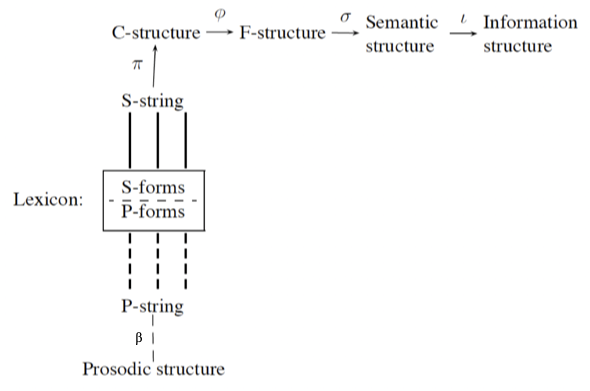
\includegraphics[scale=.5]{figures/Morphology/Dal-My-5.png}
  \caption{Proposed LFG Correspondence Architecture. From
    \citeauthor{DM11} (\citeyear{DM11}:
    178, (5); see also \citealt[409]{DLM:LFG}); used with permission.}
  \label{fig:Dal-My-5}
\end{figure}
%
A sample lexical entry for \aword{dogs} from \citet[67,~(3)]{dalrymple15} is shown
here:\footnote{This simplified lexical entry sets information
  structure aside; see \citet[66]{dalrymple15}.}

\ea \label{ex:dog-lex-fancy}
  \begin{tabular}[t]{ll}
    \begin{tabular}[t]{l}
      \emph{s-form}\\\hline
      \emph{c-structure category}\\
      \emph{f-description}\\\\\hline
      \emph{p-form}
    \end{tabular}
    & \fbox{%
      \begin{tabular}[t]{lcl}
        ($\bullet$ \feat{fm}) & $=$ & dogs\\
        $\lambda$($\pi$($\bullet$)) & $=$ & N\\
        (\UP\PRED) & $=$ & \predvall{dog}\\
        (\UP\NUM) & $=$ & \val{pl}\\\hdashline
        /dɔgz/
      \end{tabular}}
  \end{tabular}
\z
%
It is convenient to represent the information in lexical entries as a relation
\citep[67~(4)]{dalrymple15}:
%
\ea
$\mathcal{L}$$\langle$s-form, p-form, category, f-description$\rangle$
\z
%
The particular information in \exrr{dog-lex-fancy} can therefore
compactly be represented as \citep[67~(5)]{dalrymple15}:
%
\ea \label{ex:dog-lex-compact}
$\mathcal{L}$$\langle$dogs, /dɔgz/, N, \{(\UP\PRED) $=$
  \predvall{dog}, (\UP\NUM) $=$ \val{pl}\}$\rangle$
\z
%
This lexical entry generates the structures and correspondences in
\figref{fig:dalrymple15-dogs-strucs}.

\begin{figure}
  \centering
  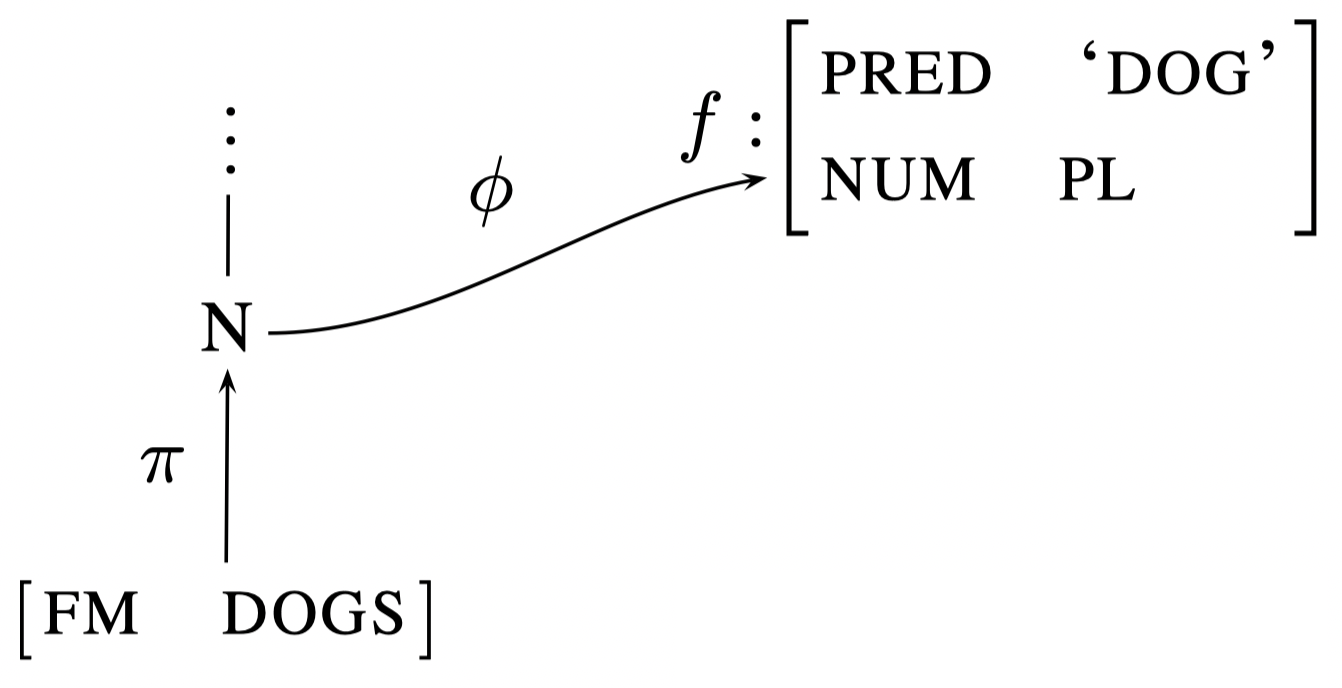
\includegraphics[scale=.25]{figures/Morphology/Dal15-2.png}
  \caption{\aword{Dogs}, contributions to the s-string, c-structure,
    and f-structure. Adapted from \citet[66,~(2)]{dalrymple15}; used with permission.}
  \label{fig:dalrymple15-dogs-strucs}
\end{figure}

\citet[68]{dalrymple15} assumes, following \citet{spencer13}, that a
\aterm{lexemic entry} consists of information about the form of the
root (and any non-predictable alternations), any syntactic information
and requirements, a representation of the semantics of the lexeme, and
an arbitrary unique lexemic index. \citet[68,~(7)]{dalrymple15} therefore defines
a lexemic entry as follows:
%
\ea
\aterm{Lexemic entry}\\ $\langle$root \& idiosyncratic stem
  forms, f-description, lexemic index$\rangle$
\z
%
She gives the following particular examples \citep[68~(8--9)]{dalrymple15}:
\ea
\ea $\langle$\{\amg{root}: dog\}, \{\,(\UP\PRED) $=$ \predvall{dog}\,\}, \amg{dog1}$\rangle$
\ex $\langle$\{\amg{root}: child; \amg{stem1}: children\}, \{\,(\UP\PRED) $=$ \predvall{child}\,\}, \amg{child1}$\rangle$
\z\z
%
The question is how these lexemic entries interact with the
morphological component  to produce complete lexical
entries. For example, how does the lexemic entry for \ali{dog1}
produce the lexical entry \exrr{dog-lex-compact}?

The answer is illustrated in the diagram in
\figref{fig:dalrymple15-15}. The realization of the s-string form
(\aterm{s-form}) and the p-string form (\aterm{p-form}) are handled by
the morphological realization function, $R$, which also contributes
morphological features (\aterm{m-features}) based on the ID of the
lexemic entry (LI). The morphosyntactic description function, $D$,
uses the m-features to represent the syntactic category and
morphologically contributed f-description. The final lexical entry has
the s-form and p-form that are computed by the realization function
$R$ (based on the m-features), the syntactic category that is computed by
the description function $D$ (again based on the m-features), and the
f-description that is the union of the lexically contributed
f-description from $LE$ and the morphologically contributed
f-description from $D$.

The relations between the different elements can be illustrated in a
logic-pro\-gram\-ming-style representation, as in
\figref{fig:dalrymple15-15-logic}. This representation reveals some
redundancy. In particular, it's not clear why $R$ and $D$ each need
access to both the lexemic index (LI) and the set of m-features (M),
especially given that M must be computed based on LI. A more
streamlined representation would eliminate LI from $D$. It would
certainly be theoretically elegant if the set of m-features was
sufficient to determine the category C and the morphologically
contributed f-description G. However, there are empirical cases that
show that $D$ must be directly conditioned on LI, such as the
syntactically singular but morphologically plural \aword{measles}
\citep[75]{dalrymple15}.
% \footnote{We still don't understand one aspect, though, which is that
% nothing makes use of Root in the lexemic entry. In other words, it
% seems that the lexemic index is sufficient and that the Root
% coordinate is surplus. Alternatively, one could imagine Root being
% used everywhere that LI is currently used and eliminating LI instead.}

As we mentioned above, \citegen{dalrymple15} model is not a theory of
morphology, but rather a theory of the interface between syntax and
morphology. Nevertheless, it is most compatible with a morphological
theory that is \aterm{lexemic}, is \aterm{Word-and-Paradigm}, and 
assumes \aterm{Strong Lexicalism}.  

%
\begin{figure}[htb]
  \centering
  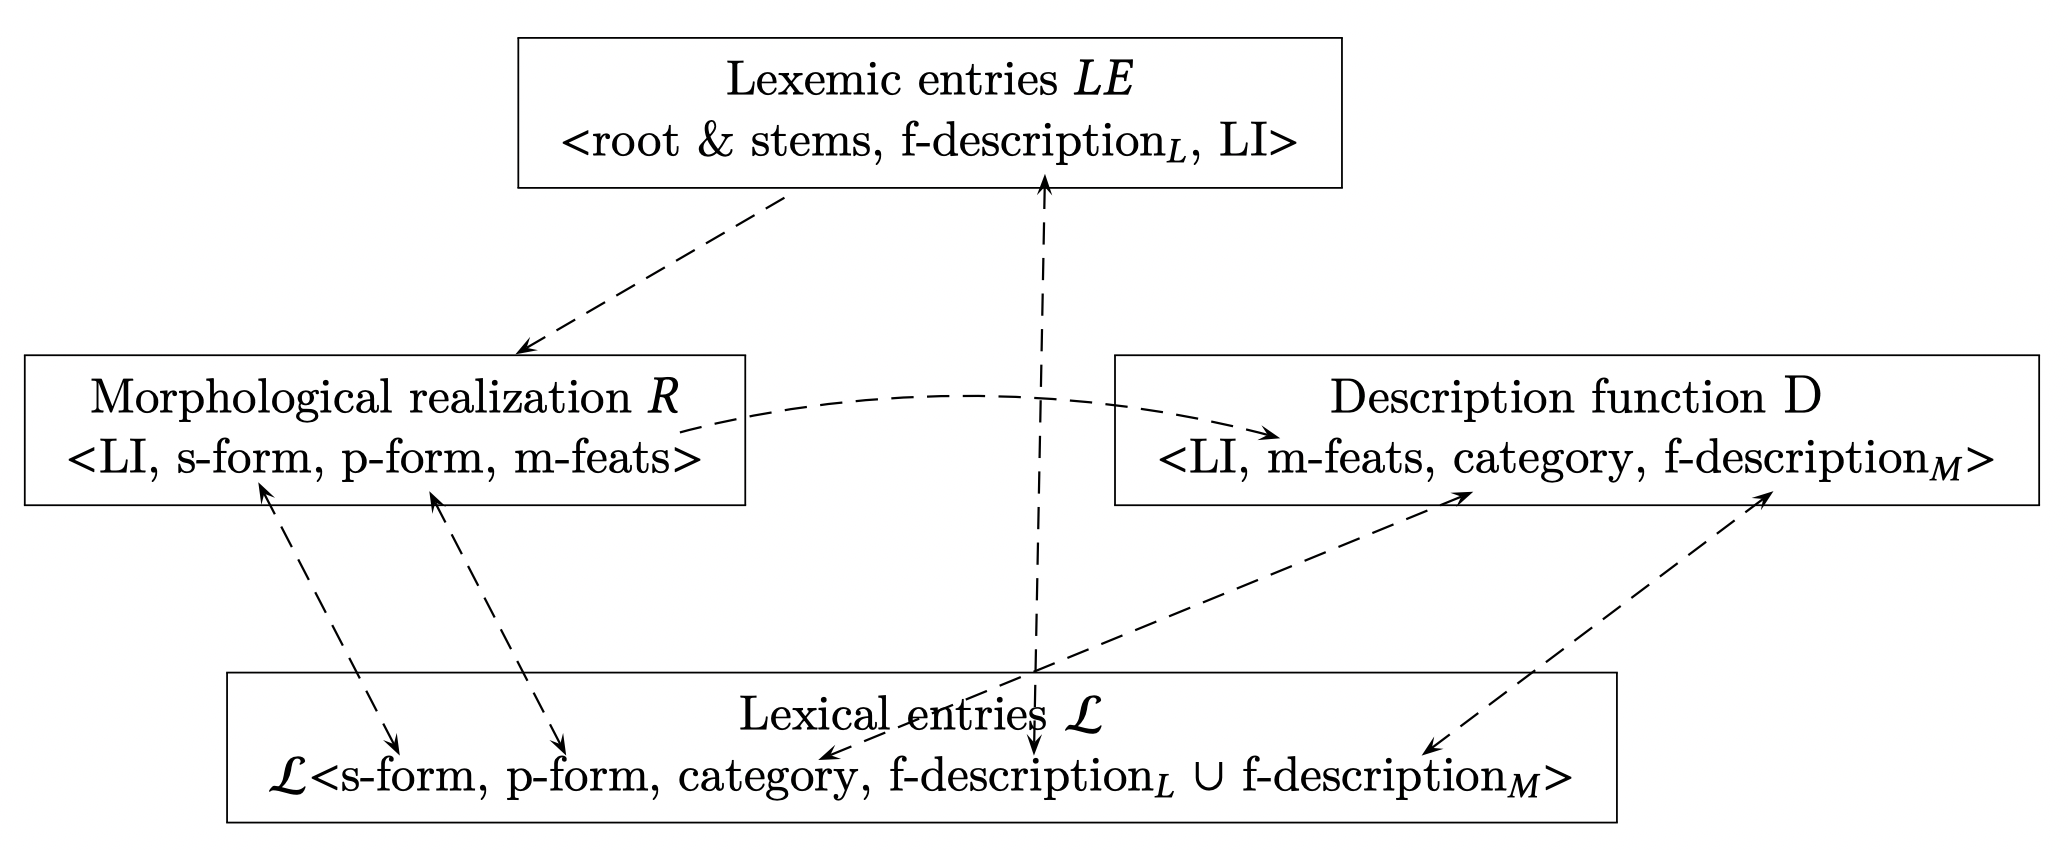
\includegraphics[scale=.325]{figures/Morphology/Dal15-15.png}
  \caption{How the set of lexical entries, $\mathcal{L}$, is computed
    from the set of lexemic entries, $LE$, using a morphological
    realization function, $R$, and a description function, $D$
    \citep[70~(15); used with permission]{dalrymple15}}
  \label{fig:dalrymple15-15}
\end{figure}
 
\begin{figure}[htb]
  \centering
  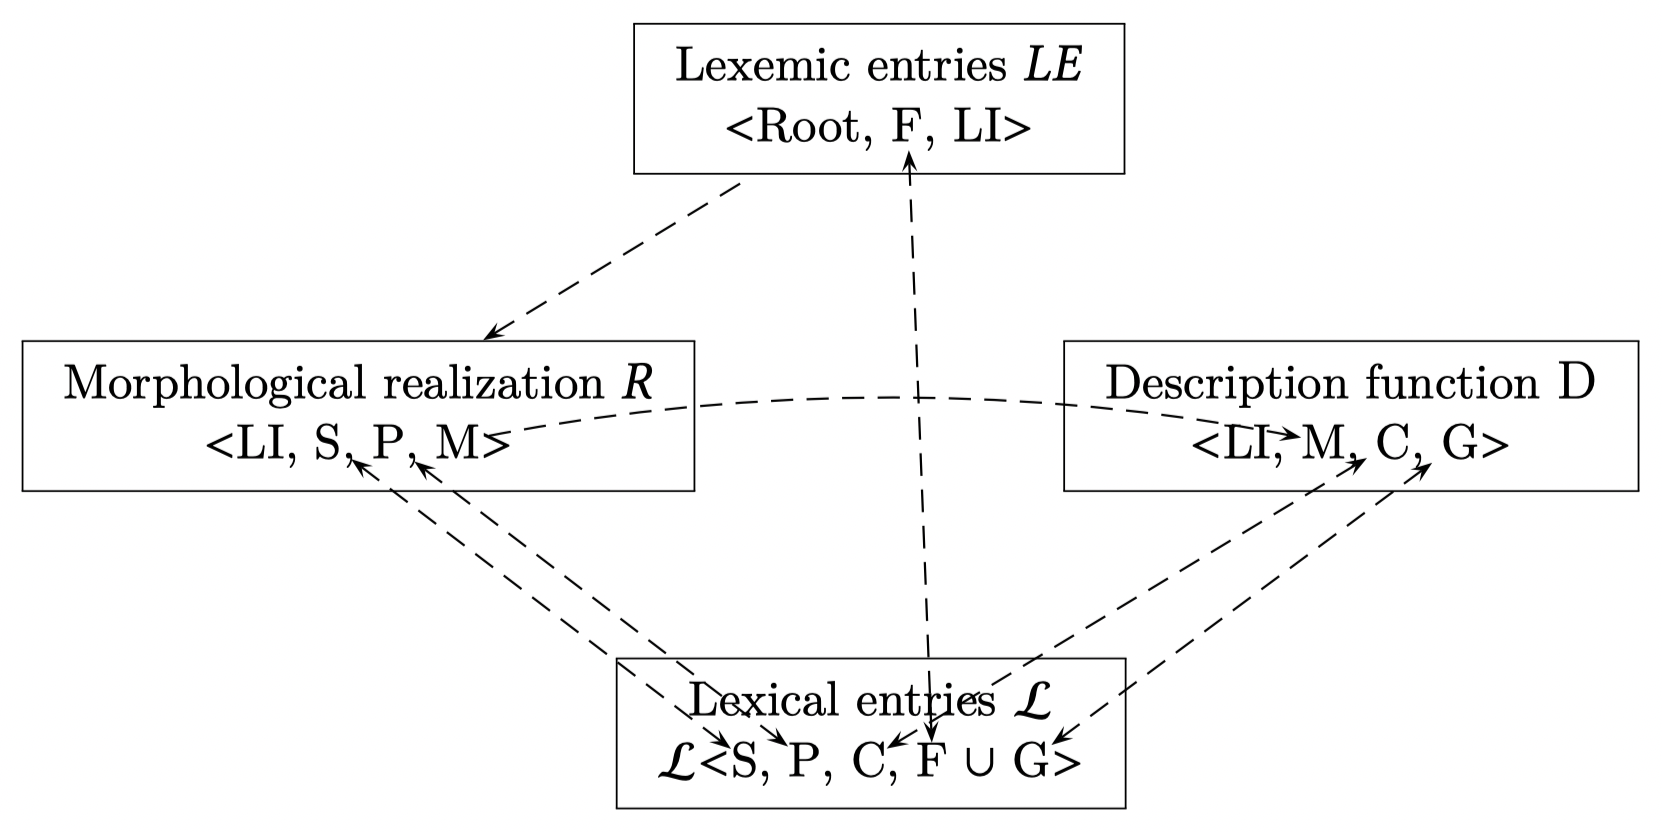
\includegraphics[scale=.325]{figures/Morphology/Dal15-15-alt.png}
  \caption{Logic-programming-style representation of the relations
    between $\mathcal{L}$, $LE$, $R$, and $D$}
  \label{fig:dalrymple15-15-logic}
\end{figure}

\subsection{M-structure}
\label{sec:Morph:m-structure}

As noted above, \citet{dalrymple15} sees her framework as a general framework for
realizational morphology and it is a feature of the approach that it
is very much backwards-compatible with existing LFG proposals about
morphological conditioning of syntax, such as the proposals for adding a
m(orphological)-structure to  the Correspondence Architecture proposed by
\citet{buttetal96} and \citet{FrankZaenen2004}, which are both LFG
accounts of affix ordering restrictions (e.g., English \ascare{affix
  hopping}). The main distinction between the two
proposals is that the first holds that m-structure is projected
from c-structure \citep{buttetal96}, whereas the second holds that
m-structure is projected from f-structure \citep{FrankZaenen2004}.

The \aterm{morphological entry} (m-entry), i.e. instance of $R$, based
on \citeauthor{buttetal96} for \aword{swimming} is shown here:
%
\ea \label{ex:m-entry-swimming}
  $R$$\langle$\amg{swim1}, swimming, /swɪmɪŋ/, \{\amg{m-cat:verb},
  \amg{m-vform:prespart}\}$\rangle$
\z
%
The relevant $D$ mapping would then be:
%
\ea \label{ex:swimming-butt} \amg{m-vform:prespart}\ $\overset{D}{\Rightarrow}$\
  \{(\amother$_\mu$\ \amg{vform}) $=$ \amg{prespart}, (\UP~\feat{aspect}) $=$ \val{prog})\}
\z
%
Given the same m-entry in \exrr{m-entry-swimming}, the relevant $D$
mapping based on \citeauthor{FrankZaenen2004} would instead be:
%
\ea
\amg{m-vform:prespart}\ $\overset{D}{\Rightarrow}$\
  \{($\phi$(\amother)$_\mu$\ \amg{vform}) $=$ \amg{prespart}, (\UP~\feat{aspect}) $=$ \val{prog})\}
\z
%
We have represented things this way for maximum comparability with \exrr{swimming-butt}, but
$\phi(\amother)$ is just \Up, so we could have written \Up$_\mu$
instead:
%
\ea
\amg{m-vform:prespart}\ $\overset{D}{\Rightarrow}$\
  \{(\Up$_\mu$\ \amg{vform}) $=$ \amg{prespart}, (\UP~\feat{aspect}) $=$ \val{prog})\}
\z
%
Note that there are other differences between the
\citeauthor{buttetal96} theory and the \citeauthor{FrankZaenen2004}
theory, but we've kept things as simple as possible for direct
comparison. See \citet{dalrymple15} for further details regarding both
of these approaches to m-structure. It's important to realize, though,
that m-structure concerns morphological conditioning on syntactic
order and is not a theory of morphology per se. However, we have seen
that the \citet{dalrymple15} framework, which \emph{can} provide the
foundation for a theory of morphology, accommodates both
approaches. This demonstrates the \citeauthor{dalrymple15} framework's
generality. M-structure is most compatible with a morphological theory
that is \aterm{lexemic}, is \aterm{Word-and-Paradigm}, and assumes
\aterm{Strong Lexicalism}.

% In sum, m-structure \citep{buttetal96,FrankZaenen2004} is not a theory of
% morphology, but rather a theory of the interface between syntax and
% morphology. Nevertheless, 

\section{Realizational morphology and LFG}
\label{sec:Morph:real-morph-lfg}

As noted in \sectref{sec:Morph:incr-vs-real}, realizational
morphology is done today in three major ways:
%
\begin{enumerate}
\item The word-based approach, such as Paradigm Function Morphology
  \citep{Stu01,stump16,spencer13}.
  % and other Word-and-Paradigm
  % aproaches \citep{blevins18}.    
\item The morpheme-based approach, such as  Distributed Morphology
  \citep{hallemarantz} and Nanosyntax \citep{Sta09,caha09}
\item The construction-based approach, such as Construction Morphology
\citep{Booij2010}  or Optimal Construction
  Morphology \citep{caballero08}
\end{enumerate}
%
To our knowledge, neither Construction Morphology nor Optimal
Construction Morphology has been interfaced with LFG, so we set them 
aside here. We focus in particular on PFM and DM interfaces to
LFG. PFM and LFG have a history going back at least to
\citet{sadler2004projecting}. There has also been renewed interest in
PFM+LFG \citep{dalrymple15,DLM:LFG}, as well as recent interest in
DM+LFG
\citep{Melchin2020,asudeh;ea21,everdell:beyond,asudeh;siddiqi-lfg22}.


% \subsubsection{Word-based approaches}
\subsection{LFG interfaced with PFM}
\label{sec:Morph:lfg-pfm}

The first attempts to interface LFG with Paradigm Function Morphology
\citep{Stu01,stump16,spencer13} were undertaken by
\citet{sadler-nordlinger2004,SadlNord2006} to account for highly
complex case-stacking in certain Australian languages and by
\citet{ackerman;stump04} to deal with the general problem of
\aterm{periphrasis}. However, the complexity of the data and
phenomena involved 
precluded either of these collaborations from simultaneously providing
a general theory of realizational morphology for LFG. As we have seen,
steps in that direction were taken by \citet{dalrymple15} and
\citet{DLM:LFG}. Although the \citeauthor{dalrymple15} framework is
general and not specifically geared towards PFM, there is a deep
compatibility between LFG's version of Strong Lexicalism, the Lexical
Integrity Principle (see \exrr{lip} below), and PFM. 
% (or some other Word and Paradigm
% morphology; \citealt{blevins18}).
As \citet{dalrymple15} presumably wishes
to preserve Lexical Integrity/Strong Lexicalism --- the traditional/default stance
in LFG theory --- then it is natural that she envisages a word-based
morphology. \citet[22]{thomas21} aptly sums up this underlying
compatibility as follows:
%
\begin{quote}
  Unlike many other theories of morphology, the concept of a
  `morpheme' is irrelevant to PFM: there is no conception of a
  form-meaning pair below the level of the word, as only fully
  inflected forms are associated with morphosyntactic property
  sets. This aligns with the Lexical Integrity Principle of LFG, by
  which terminal nodes must correspond to fully inflected words,
  rather than to morphemes or other sub-word elements.
\end{quote}
%
If one wishes to retain LFG's Strong Lexicalism, such
that the fundamental building blocks of syntax are words, then it
makes sense to interface the syntax with a word-based theory of
morphology. And PFM is arguably the most formally well-developed
realizational, word-based morphological theory, making it a
natural choice. Indeed \citet[23]{thomas21} notes in passing that
PFM's rigorous formalization offers another natural point of
compatibility between PFM and LFG: \aquoot{PFM also shares with LFG a
  commitment to being formally explicit and rigorously testable, as
  well as computationally implementable.} 


PFM's fundamental claim is that lexemes are represented as pairs of a form
and a set of morphological properties (captured as features). Thus, in
$\langle$X,$\sigma$$\rangle$, X is the form and $\sigma$ is the set
of properties. A paradigm function relates the lexeme to its
inflectional realizations, by mapping the input form to an output form
given the morphological properties:
% Thomas 2021: 22, (7)
\ea \label{ex:par-func}
$\langle$X,$\sigma$$\rangle$ $\overset{f}{\longrightarrow}$ $\langle$Y,$\sigma$$\rangle$
\z
%
These paradigm functions are defined in terms of realization rules,
which consist of \aterm{rules of exponence} and \aterm{rules of
  referral}. Rules of exponence realize the property set
directly. Rules of referral instead refer the realization of their
property sets to one or more other realization rules. There is a 
limited number of additional rule types; furthermore \citeauthor{Stu01}'s
\citeyearpar{Stu01} notion of paradigm has been refined in
\citet{stump16}, which is typically called PFM2. However, this simple
account will have to serve our purposes.

The realization rules in PFM are arranged into ordered rule
\aterm{blocks}; however, there is no ordering within blocks. 
% The
% ordering of blocks results in the ordering of morphemes in the overall
% output.
Given Panini's principle, the effect of block ordering mimics concatenation, but
allows a morphologically synthetic form
(\aterm{portmanteau}\footnote{Note that, in this literature, the term
  \aterm{portmanteau} has a more restrictive use than how we use it
  here. What we
  have been calling a portmanteau would be called \aterm{cumulative
    exponence}. }) to block
a morphologically analytic form. Selection
of the correct rule in any given block is governed by Paninian
blocking: the most specific rule that can apply in any given rule block
must apply. PFM also assumes a principle called the Identity Function
Default (IFD), which states that the identity function is a member of every
rule block: If no other rule applies, the output is identical to the
input. 

This is exemplified by the following rules for Swahili future and past
tenses \citep[402--403]{stewart;stump07}, which \citet[22]{thomas21}
presents in simplified form.\footnote{The simplification does not
  account for all the nuances of the paradigms that are captured by
  the rules in \citet{stewart;stump07}.} We have adapted the
representation for maximal consistency with \exrr{par-func} above.
%
\ea
  \scalebox{0.95}{
  \begin{tabular}[t]{@{}ll@{~$\longrightarrow$~}l@{}}
    Block A & \apf[$\sigma$:\aset{\amg{cat}:verb,\amg{tns}:fut}]{X} &
                                                             \apf{\aword{ta}X}\\
    & \apf[$\sigma$:\aset{\amg{cat}:verb,\amg{tns}:past}]{X} & \apf{\aword{li}X}\\
    & \apf[$\sigma$:\aset{\amg{cat}:verb,\amg{pol}:neg,\amg{tns}:past}]{X} &
                                                                    \apf{\aword{ku}X}
    \\[1ex]
    Block B &
              \apf[$\sigma$:\aset{\amg{cat}:verb,\amg{agr}(su):\aset{\amg{pers}:1,\amg{num}:sg}}]{X} &
                                                                                            \apf{\aword{ni}X}\\
    & \apf[$\sigma$:\aset{\amg{cat}:verb,\amg{agr}(su):\aset{\amg{pers}:2,\amg{num}:sg}}]{X} &
                                                                                            \apf{\aword{u}X}\\
    &
      $\langle$X,$\sigma$:\{\amg{cat}:verb,\amg{agr}(su):\begin{tabular}[t]{@{}l@{}}\aset{\amg{pers}:3,\amg{num}:sg},\amg{gen}:\aset{1,2}\}$\rangle$
                                \end{tabular}
                                                           &
                                                             \apf{\aword{a}X}\\
    &
      \apf[$\sigma$:\aset{\amg{cat}:verb,\amg{agr}(su):\aset{\amg{pers}:1,\amg{num}:pl}}]{X}
                                                           &
                                                             \apf{\aword{tu}X}\\
    &
      \apf[$\sigma$:\aset{\amg{cat}:verb,\amg{agr}(su):\aset{\amg{pers}:2,\amg{num}:pl}}]{X} & \apf{\aword{m}X}\\
    &
      $\langle$X,$\sigma$:\{\amg{cat}:verb,\amg{agr}(su):\begin{tabular}[t]{@{}l@{}}\aset{\amg{pers}:3,\amg{num}:pl},\amg{gen}:\aset{1,2}\}$\rangle$
                                \end{tabular}
                                                           &
                                                             \apf{\aword{wa}X}
    \\[1ex]
        Block C &
              \apf[\aset{\amg{cat}:verb, \amg{pol}:neg}]{X} & \apf{\aword{ha}X}\\
  \end{tabular}
  }
\z
%
Recall that the identity function, \apf{X} $\longrightarrow$ \apf{X},
is a member of every rule block, according to the IFD. Thus, we see
for example, that the negated third singular past tense form is correctly predicted
to be \aword{ha-a-ku}-\amg{root} and not *\aword{ha-a-li}-\amg{root}, because
the portmanteau form \aword{ku} expresses both the past tense and the
negation. From Block A, then, the third rule must be chosen. From
Block B, the third rule best expresses the features. Lastly, the
rule in Block C can apply, given the input features. The result is the
well-formed \aword{ha-a-ku}-\amg{root}, which undergoes phonological
shortening to \aword{ha-ku}-\amg{root}. 

\citet{sadler-nordlinger2004} presented an LFG interface to PFM for
case-stack\-ing in Australian languages that display that phenomenon
(e.g., Kayardild, Martuthunira, Thalanyji, Wambaya). \citet{SadlNord2006}
subsequently presented the actual PFM morphology, i.e. realization, of
case-stacking morphology. The two papers together constitute an
instance of LFG interfaced with
PFM. \citet[172--180]{sadler-nordlinger2004} provide a detailed
analysis of the following example from Martuthunira
\citep[60,~(3.15)]{dench1995}:
%
\ea \label{ex:sad-nor} Martuthunira\\
\gll
    Ngayu nhawu-lha ngurnu tharnta-a mirtily-marta-a thara-ngka-marta-a. \\
    I saw-\amg{pst} that.\amg{acc} euro-\amg{acc}
    joey-\amg{prop}-\amg{acc}
    pouch-\amg{loc}-\amg{prop}-\amg{acc}\\
\glt 1 saw the euro with a joey in (its) pouch.
\z
%
\citet[174,~(28)]{sadler-nordlinger2004} provide the following lexemic
entry\footnote{We use the terminology of \citealt{dalrymple15}; see
  \sectref{sec:Morph:interface} above.} for the word
\aword{tharangkamartaa} in \exrr{sad-nor}:
%
\ea
$\langle$\aword{thara}, \aset{Case$_C$: \amg{loc},
    \aset{Case$_C$: \amg{prop}, \aset{Case$_C$: \amg{acc}}}}$\rangle$
\z
%
\citet[174,~(25)]{sadler-nordlinger2004} provide the following interpretations of
these case features:\footnote{Their table does not include \amg{acc}
  but what its entry should be is clear from their (30)
  \citep[175]{sadler-nordlinger2004}. Also, we have adjusted for the
  feature \feat{adj} being set-valued by using the symbol $\in$.}
%
\ea 
  \begin{tabular}[t]{@{}l|l@{}}
    M-feature & F-description \\\hline
    Case$_C$: \amg{loc} &
                          \begin{tabular}[t]{@{}l@{}}
                            (\UP\CASE) $=$ \val{loc}\\
                            (\feat{adj}\textsubscript{\textit{loc}}
                            $\in$ \Up)
                          \end{tabular}\\
    Case$_C$: \amg{prop} &
                          \begin{tabular}[t]{@{}l@{}}
                            (\UP\CASE) $=$ \val{prop}\\
                            (\feat{adj}\textsubscript{\textit{prop}} $\in$ \Up)
                          \end{tabular}\\
    Case$_C$: \amg{acc} &
                          \begin{tabular}[t]{@{}l@{}}
                            (\UP\CASE) $=$ \val{acc}\\
                            (\feat{obj} \Up)
                          \end{tabular}\\
  \end{tabular}
\z
%

In the \citet{dalrymple15} notation this would be:\footnote{The (\UP\NUM) $=$ \val{sg} part of
  the f-description occurs by default, following the assumption in
  \citet[76]{dalrymple15} that singular number is the default for nouns
  (i.e., \feat{m-cat}:\amg{n} in the absence of \feat{m-num}
  introduces the f-description \aset{(\UP\NUM) $=$ \val{sg}}).\label{fn:dal-def}}
%
\ea 
  $LE$$\langle$\aset{\amg{root}: pouch}, \aset{(\UP\PRED) $=$
    \predvall{pouch}}, \amg{pouch1}$\rangle$
  \\[1ex]
  $R$$\langle$%
  \begin{tabular}[t]{@{}l@{}}
    \amg{pouch1}, tharangkamartaa,
    /{t̪araŋkamaʈaa}/,\\
    m-features:\aset{\amg{m-cat}:\amg{n}, \amg{m-case}: \amg{loc},
    \aset{\amg{m-case}: \amg{prop}, \aset{\amg{m-case:}
    \amg{acc}}}}$\rangle$
  \end{tabular}
  \\[1ex] 
  $D$$\langle$\amg{pouch1}, m-features, N,
  \begin{tabular}[t]{@{}l@{}}
    (\UP\NUM) $=$ \val{sg}\\
    (\UP\CASE) $=$ \val{loc}\\
    (\feat{adj}\textsubscript{\textit{loc}} $\in$ \Up)\\
    ((\feat{adj}\textsubscript{\textit{loc}} $\in$ \Up) \feat{case}) $=$
    \val{prop}\\
    (\feat{adj}\textsubscript{\textit{prop}} $\in$ 
    \feat{adj}\textsubscript{\textit{loc}} $\in$ \Up)\\
    (((\feat{adj}\textsubscript{\textit{prop}} $\in$
    \feat{adj}\textsubscript{\textit{loc}} $\in$ \Up)) \feat{case}) $=$
    \val{acc}\\
    (\feat{obj} \feat{adj}\textsubscript{\textit{prop}} $\in$
    \feat{adj}\textsubscript{\textit{loc}} $\in$ \Up)$\rangle$
  \end{tabular}
  \\[1ex]
  $\mathcal{L}$$\langle$%
  \begin{tabular}[t]{@{}l@{}}
    tharangkamartaa,
    {/t̪araŋkamaʈaa}/,\\
    N,
    \{\begin{tabular}[t]{@{}l@{}}
      (\UP\PRED) $=$ \predvall{pouch}\\
   (\UP\NUM) $=$ \val{sg}\\
    (\UP\CASE) $=$ \val{loc}\\
    (\feat{adj}\textsubscript{\textit{loc}} $\in$ \Up)\\
    ((\feat{adj}\textsubscript{\textit{loc}} $\in$ \Up) \feat{case}) $=$
    \val{prop}\\
    (\feat{adj}\textsubscript{\textit{prop}} $\in$
    \feat{adj}\textsubscript{\textit{loc}} $\in$ \Up)\\
    (((\feat{adj}\textsubscript{\textit{prop}} $\in$
    \feat{adj}\textsubscript{\textit{loc}} $\in$ \Up)) \feat{case}) $=$
    \val{acc}\\
    (\feat{obj} \feat{adj}\textsubscript{\textit{prop}} $\in$
    \feat{adj}\textsubscript{\textit{loc}} $\in$ \Up)\}$\rangle$
    \end{tabular}
  \end{tabular}
\z
%
This complex lexical entry
$\mathcal{L}$\textsubscript{\aword{tharangkamartaa}} licenses the
following f-structure:
%
\eabox{\attop{%
  \avm[style=fstr]{
    [obj & [case & acc\\
      adj\textup{\textsubscript{\textit{prop}}} & 
      \{[case & prop\\
        adj\textup{\textsubscript{\textit{loc}}} &
        \{ [pred & \predvall{pouch}\\
             num & sg\\
             case & loc]\}]
      \}]
      ]
    }
  }
}
%
Thus, we can observe that the \citet{dalrymple15} notation accurately
reconstructs the intended f-structure from
\citet[178,~(36)]{sadler-nordlinger2004}.\footnote{Modulo our use of $\in$, which
they simplify away, and the [\feat{num} \val{sg}], which comes from
\citeauthor{dalrymple15}'s default; see footnote~\ref{fn:dal-def} above.}

However, some work remains to be done. How is the realization of
\aword{tharangkamartaa} determined based on the root, lexemic ID, and
the m-features? The \citet{dalrymple15} framework is silent on this issue,
because it is meant to be a \emph{general} interface between LFG
syntax and realizational morphology. In order to preserve its
generality, the framework remains silent on the question of
exponence. As mentioned above, \citet{SadlNord2006} provide a
PFM account, which we can plug into the \citeauthor{dalrymple15}
framework. Adapting their proposal
\citep[471,~23]{sadler-nordlinger2004} --- which in any case is for
Kayardild,  not Martuthunira --- we get the following case rule block,
using the \citet{dalrymple15} $R$ function:
%
\ea
\ea    
$R$$\langle$%
  \begin{tabular}[t]{@{}l@{}}
    \amg{pouch1}, tharangka,
    /{t̪araŋka}/, \\
    \aset{\amg{m-cat}:\amg{n}, \amg{m-case}: \amg{loc}}$\rangle$
  \end{tabular}
\ex $R$$\langle$%
  \begin{tabular}[t]{@{}l@{}}
    \amg{pouch1}, tharangkamarta,
    /t̪araŋkamaʈa/, \\
    \aset{\amg{m-cat}:\amg{n}, \amg{m-case}: \amg{prop}}$\rangle$
  \end{tabular}
\ex $R$$\langle$%
  \begin{tabular}[t]{@{}l@{}}
    \amg{pouch1}, tharangkamartaa,
    /t̪araŋkamaʈaa/, \\
    \aset{\amg{m-cat}:\amg{n}, \amg{m-case}: \amg{acc}}$\rangle$
  \end{tabular}
\z\z
%
The effect of these functions on the s-form can be captured in the
following simplified PFM representation, based on
\exrr{par-func}.\footnote{Note that the simplified formalization in
  \exrr{sad-nor-par1} does not account for the set-based embedding in
  \exrr{sad-nor} above. But it should be easy enough to replace
  the second coordinate of the input to their function with 
  \cons{contains}($f$), where \cons{contains} is a function that
  recursively searches $\sigma$ for its argument, $f$, a feature,
  e.g. \amg{m-case:loc}.}
%
\ea\label{ex:sad-nor-par1}
  \begin{tabular}[t]{l@{~$\longrightarrow$~}l}
    \apf[$\sigma$:\aset{\amg{m-cat}:\amg{n}, \amg{m-case}:\amg{loc}}]{X} & \apf{X\aword{ngka}}\\
    \apf[$\sigma$:\aset{\amg{m-cat}:\amg{n}, \amg{m-case}:\amg{prop}}]{X} & \apf{X\aword{marta}}\\
    \apf[$\sigma$:\aset{\amg{m-cat}:\amg{n}, \amg{m-case}:\amg{acc}}]{X} & \apf{X\aword{a}}
  \end{tabular} 
\z
%
In other words, in the context of the features \amg{m-cat:n} and
\amg{m-case:loc}, the input exponent becomes extended with additional
morphological information, the suffix \aword{ngka}. In the context of the features \amg{m-cat:n} and
\amg{m-case:prop}, the input exponent becomes extended with additional
morphological information, the suffix \aword{marta}. And, in the context of the features \amg{m-cat:n} and
\amg{m-case:acc}, the input exponent becomes extended with additional
morphological information, the suffix \aword{a}. 

In sum, much work in LFG has adopted Paradigm Function Morphology as
its morphological theory. 
PFM is an \aterm{inferential-realizational}
theory of morphology. It is \aterm{lexemic}, it is \aterm{Word-and-Paradigm},
and it assumes \aterm{Strong Lexicalism}.


\subsection{The targets of exponence}

What realizational theories have in common is that morphology realizes
things; what they don't have in common is what those things are. In a
paradigm model, like PFM, morphology realizes a lexeme and a valuation
of a fixed set of attributes. It must be a \emph{fixed} set of
attributes, by definition of a paradigm. As \citet{spencer13} notes:
%
\begin{quote}
  On this [\ldots] conception we abstract away from actual word forms and just
  consider the set of oppositions or contrasts that are available in
  principle to a lexeme.  \citep[9]{spencer13}
\end{quote}
%
\aquoot{The set of cells embodying the set of oppositions open to a lexeme} is
what \citet[9]{spencer13} calls the \aterm{property paradigm}. It's
\emph{this} abstraction, the property paradigm,  that is realized by
word forms (the \aterm{form paradigm}) in
what \citeauthor{spencer13} calls the \aterm{form-property paradigm} \citep[9]{spencer13}. In
this kind of conception, in order to preserve Strong Lexicalism one must
simply have an intervening function that maps a lexeme to a syntactic
word: 
\ea \label{ex:spencer-mapping}
  form-property paradigm $\overset{f}{\longrightarrow}$ set of
  instantiated lexical entries for syntax
  % \begin{tabular}[t]{lcl}
  %   & & form paradigm\\
  %   &  \overset{$f$}{$\nearrow$} &  \\ 
  %   property paradigm & &\\
  %   &  $\searrow$ & \\
  %   & & set of instantiated lexical entries for syntax 
  % \end{tabular}
\z
%
The mapping $f$ can be a structured mapping, if there are features of
the mapping itself that the grammar needs to refer to. This could be
represented as an attribute-value matrix. In other words, m-structure
(see above) is one possible characterization of the structured mapping
$f$. And an AVM is also indeed how \citet{spencer13} models the
structured mapping $f$; see \figref{fig:spencer}. This paradigm shows
the lexeme \amg{delat}$'$ \attrns{make} from Russian, which has
stem alternants in the present (\aword{delaj-}), infinitive
(\aword{dela-}), and predicative adjective (\aword{delal-}).

\begin{figure}[b]
  \centering
  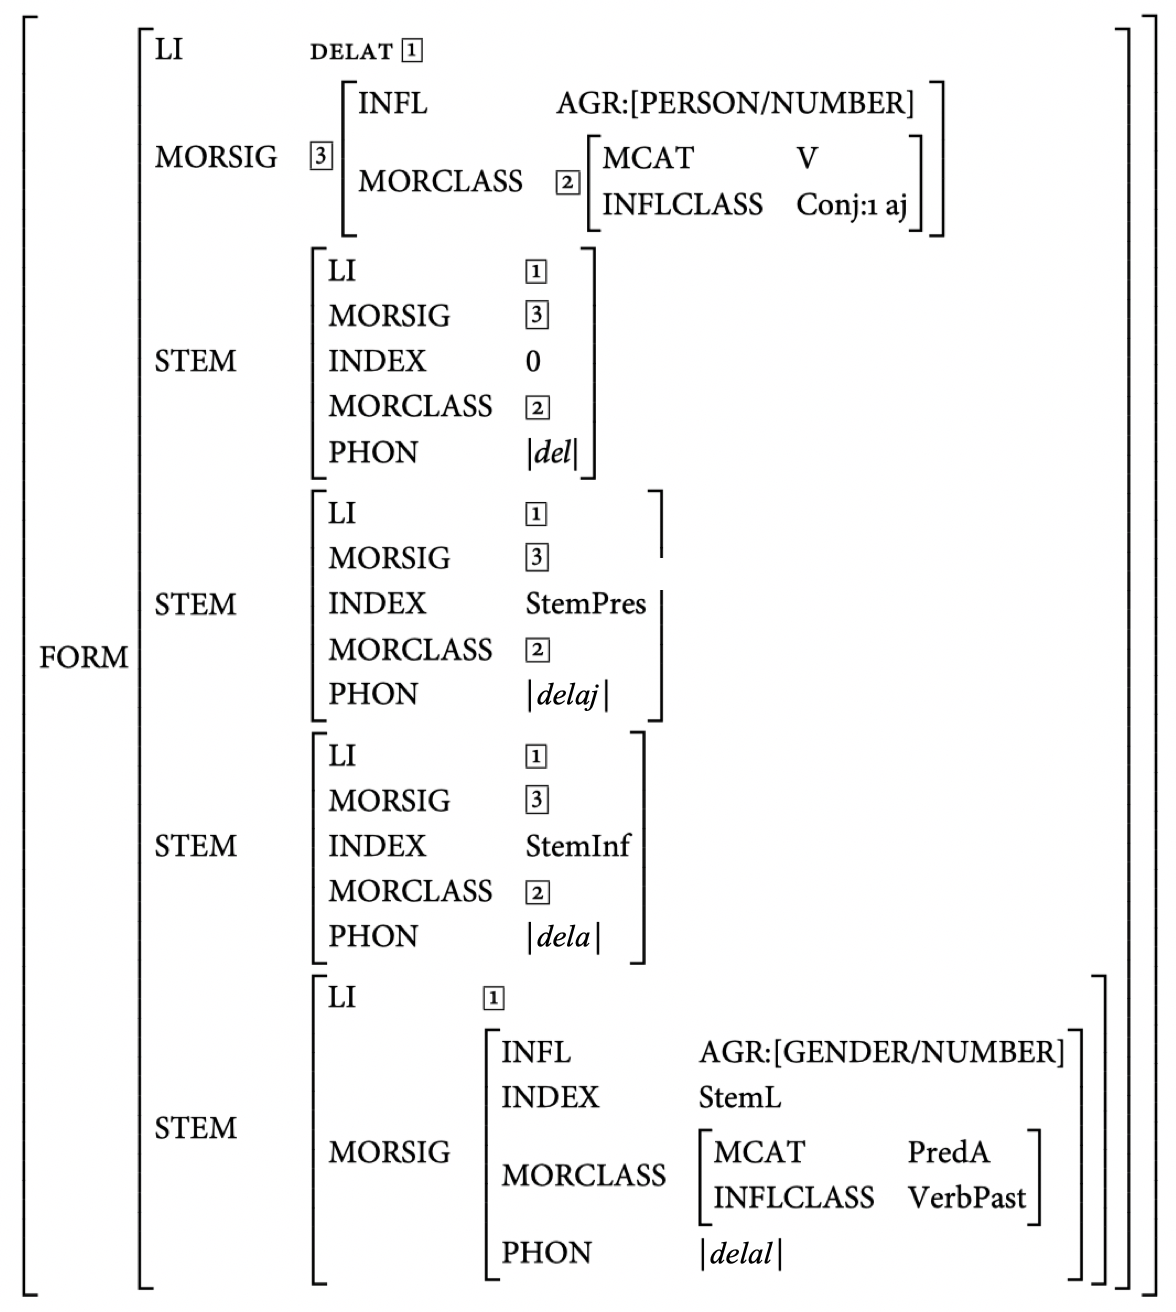
\includegraphics[scale=0.45]{figures/Morphology/Spencer13-263.png}
  \caption{The form-property paradigm for Russian \amg{delat}$'$
    \attrns{make}. From \citet[263,~(56)]{spencer13}; used with permission.}
  \label{fig:spencer}
\end{figure}

\citet{ackerman;stump04} make an antecedent proposal to that of
\citet{spencer13} which is very similar, although not as
well-developed (as a consequence of the former being a paper and the
latter a monograph). However, it is worth reading the following
passage from \citet{ackerman;stump04} to get a different perspective
on the form-property paradigm of \citet{spencer13}, especially because
it refers more directly to LFG structures:
%
\begin{quote}
  \begin{sloppypar}
    In distinguishing a lexeme's content-theoretic aspects from its
    form-theo\-retic aspects, we will pursue an innovative conception
    of the lexicon and its relation to c-structure, f-structure, and
    morphological realization. On this conception, a language's
    lexicon is bipartite with respect to content and form: one part of
    its lexicon is its \amg{lexemicon}, whose individual entries are
    lexemes bearing lexical meanings: the complementary part is its
    \amg{radicon}, whose individual entries are roots, i.e. elements
    of form. Every member L of a language's lexemicon has an
    associated \feat{content-paradigm} C-P(L) such that each cell in
    C-P(L) consists of the pairing of L with a complete set of
    morphosyntactic properties; we refer to any such pairing as a
    \amg{CONTENT-CELL}. Crucially, content-cells represent ensembles
    of semantically interpretable information. In contrast, every
    member r of a language's radicon has an associated
    \amg{FORM-PARADigM} F-P(r) such that each cell in F-P(r) consists
    of the pairing of r with a set of differentiating morphosyntactic
    property labels; we refer to any such pairing as a
    \amg{FORM-CELL}. A language's paradigms of form-cells house the
    information necessary to deduce the morphological realization of
    the cells in that language’s content-paradigms.
    \citep[117--118]{ackerman;stump04}
  \end{sloppypar}
\end{quote}
%
\begin{sloppypar}
  \noindent Although their terminology is different, there are obvious
  correspondences with \citet{spencer13}. \citet{ackerman;stump04}
  assume that a lexicon consists of two parts. The first part is the
  \amg{lexemicon}, which \aquoot{has an associated
    \feat{content-paradigm}}. Their content-paradigm corresponds to
  \citeauthor{spencer13}'s property paradigm. The second part of the
  lexicon for \citet{ackerman;stump04} is the \amg{radicon}, which
  \aquoot{has an associated \amg{form-paradigm}}. Their form-paradigm
  corresponds to \citeauthor{spencer13}'s form paradigm. Taken
  together, then, \citegen{ackerman;stump04} lexicon is equivalent
  to a set of \citegen{spencer13} form-property paradigms. As a
  consequence, the mapping in \exrr{spencer-mapping} above also
  accurately characterizes the \citet{ackerman;stump04} proposal,
  which is about periphrasis --- when a paradigm cell is filled by 
  more than one word. Further work in this vein can be found in, e.g., 
  \citet{AckermanStumpWebelhuth2011} and \citet{Spencer15}. We have chosen to
  describe the \citet{spencer13} and \citet{ackerman;stump04} work because
  of their close connection to LFG, but PFM2 \citep{stump16} incorporates similar principles. 
\end{sloppypar}

The important takeaway here is that in lexemic morphology
there is a mapping (structured or not) from an abstract property
paradigm --- whose features are purely morphological --- to
syntax. One could imagine instead having morphology realize the
syntactic representation(s) directly, which is the approach taken in
Distributed Morphology \citep[DM;][]{hallemarantz}, and theories
like it (e.g., Nanosyntax; \citealt{Sta09}, \citealt{caha09}). This
comes at the expense of (at least some of) Strong Lexicalism, as
discussed below in reference to \exrr{lip}, but it does away with the
abstraction of the property paradigm. In a morphemic model, like DM,
morphology realizes the information in the terminals of some syntactic
representation. There will necessarily be information about syntax,
but also possibly about semantics and other aspects of grammar (if
they are modelled separately).

% \subsubsection*{♫ end interlude}

%\subsubsection{Morpheme-based approaches}
\subsection{LFG interfaced with DM}
\label{sec:Morph:lfg-dm}

\begin{sloppypar}
  In \sectref{sec:Morph:lfg-pfm}, we explored LFG paired with PFM, an
  inferential-realizational framework for morphology. In this section,
  we see LFG paired with Distributed Morphology, a
  lexical-realizational framework. This combination is called
  Lexical-Realizational Functional Grammar (\lrfg;
  \citealt{AsSi16,Melchin2020,everdell:beyond},
  \citealt{asudeh;siddiqi-nd}). \lrfg\ accomplishes this synthesis of
  LFG and DM by mapping
  information from the c-structure to a realization, or
  \aterm{exponent}, called \aterm{vocabulary structure}.
\end{sloppypar}

Importantly, \lrfg\ assumes that c-structure terminals are not
\emph{words}, but just grammatical and semantic information, with no
associated information about the form (e.g., \aterm{s-form}; see
\sectref{sec:Morph:general-framework}) included in the
c-structure. This fact, together with the fact that \lrfg\ follows DM
in postulating highly articulated morphological structure,
differentiates 
\lrfg\ c-structures from LFG c-structures. However, \lrfg\ uses the
LFG formal machinery and assumes the same kinds of annotated
c-structure rules. In \lrfg, the categorial information in c-structure
\emph{preterminals} and the other information in c-structure \emph{terminals} are realized
by \lrfg's $\nu$ correspondence function as
v(ocabulary)-structures. Since \lrfg\ assumes a version of
LFG's Correspondence Architecture \citep{kapl:89,kaplan1995formal},
the information that v-structures express is not \emph{purely}
syntactic. V-structures also express information about semantics (encoded in Glue Semantics
\aterm{meaning constructors}: see \citetv{chapters/Glue})
and can indeed express 
information structure or any other aspect of grammar that is encoded
in distinct modules in the Correspondence
Architecture. % For example, this means that the notion
% of \aterm{morphosemantics} --- a direct interface between semantics
% and morphology --- makes sense in \lrfg\ \citep{asudeh;siddiqi-lfg22}
% in a way that it does not for versions of DM based on a Minimalist
% PF/LF model. In other words, \lrfg\ is the off-spring of the marriage
% of LFG and DM. That is, \lrfg\ is \emph{both} a kind of LFG theory
% \emph{and} a kind of DM theory.

\lrfg\ seeks to add to LFG's strengths in accounting for
\aterm{nonconfigurationality}  by adding DM's strengths in accounting
for \aterm{polysynthesis}. These two properties co-occur with some
frequency in non-European languages. \lrfg\ also seeks to account for
highly agglutinative languages like Finnish and Turkish.
Additionally, because the realizational module, v-structure,
interfaces with prosodic structure, \lrfg\ draws on existing LFG work,
especially \citet{Boegel2015}, on clitic ordering and extends it to
affixation. \citet{asudeh;bogel;siddiqi-momot} develops the interface
between v-structure and p(rosodic)-structure (by the $\rho$
correspondence function) and the mapping from p-structure to the
p(honological)-string (by the $o$ correspondence function). 

% has the
%   potential to give non-transderivational prosodic explanations for
%   morpheme alignment and surface form phenomena that are typically
%   alternatively analyzed in transderivational harmonic approaches to
%   the morphology-phonology interface, such as Optimality Theory
%   \citep{PrinceSmolensky2004}. This
  
\begin{figure}[htb]
  \centering
  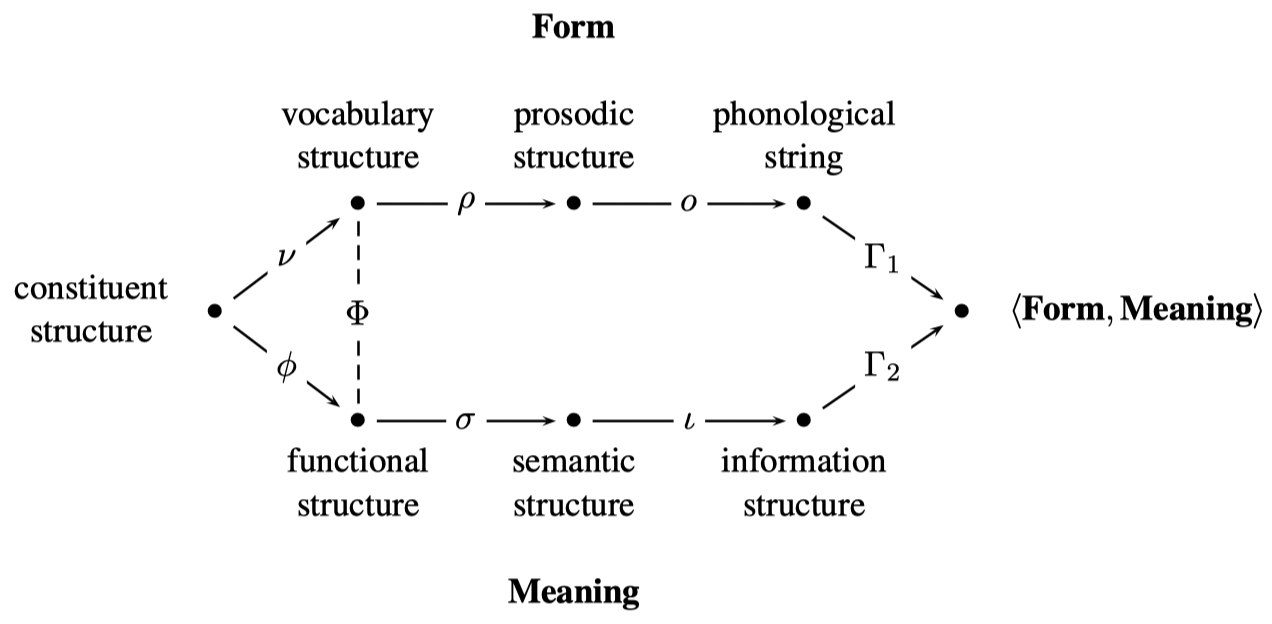
\includegraphics[scale=.55]{figures/Morphology/lrfg-corrarch.png}
  \caption{\lrfg's version of LFG's Correspondence Architecture. From
    \citet[271]{Melchin2020}; used with permission.}
  \label{fig:lrfg-corrarch}
 \end{figure}
 
 \lrfg's version of LFG's Correspondence Architecture is shown in
 \figref{fig:lrfg-corrarch}, which shows that there is a lot shared
 between \lrfg\ and LFG. However, there is no lexicon feeding the
 c-structure in \lrfg. Rather, there is a Vocabulary in \lrfg\ that
 consists of a set of mappings from n-tuples that contain categorial
 information and an f-description to vocabulary structures that
 realize the content of the input. In recent \lrfg\ work on
 morphosemantics \citep{asudeh;siddiqi-lfg22}, we suggest that, for
 the purposes of the $\nu$-mapping, the f-description could be
 usefully partitioned into a set consisting of information about
 non-f-structural aspects of the grammar (in particular, Glue meaning
 constructors for compositional semantics) and the set consisting of
 the rest of the f-description, which is information about
 f-structure.\footnote{The new third coordinate could potentially also
   include i-structural information; or perhaps this would be better
   captured in a separate fourth
   coordinate. We plan to explore this in future work.} The following
 example shows Vocabulary Items (VIs) for Ojibwe and English roots for
 \aword{see} \citep{asudeh;siddiqi-lfg22}:\footnote{We will present
   the \aterm{bridging function}, $\Phi$, shortly.}
 %
 \ea\label{ex:waab-vi} \mbox{Ojibwe} \\
   \begin{tabular}[t]{@{}lcl@{}}
     \scalebox{0.9}{
     \begin{tabular}[t]{@{}lcl@{}}
     $\langle$
     {  [\dmroot]},\  
     \ensuremath{
     {\fsfunc\left\{
     \begin{tabular}{@{}l@{}}
       (\UP\PRED) = \pred{see}\\
     \end{tabular}
     \right\}}, {\left\{\formula{\cons{see}:(\UP~\OBJ)\sig \linimp (\UP~\SUBJ)\sig \linimp \upsigb}\right\}}
     }
       $\rangle$ ~$\expone$
     \end{tabular}
     }\hspace*{-.5em}
     \aword{waab}
   \end{tabular} 
   \z
   \ea\label{ex:see-vi}
   \mbox{English} \\ \begin{tabular}[t]{@{}lcl@{}}
                       \scalebox{0.9}{
                       \begin{tabular}[t]{@{}lcl@{}}
                           $\langle$
                           { [\dmroot]},\  
                           \ensuremath{
                           {\fsfunc\left\{
                           \begin{tabular}{@{}l@{}}
                             (\UP\PRED) = \pred{see}\\
                           \end{tabular}
                           \right\}}, {\left\{\formula{\cons{see}:(\UP~\OBJ)\sig \linimp (\UP~\SUBJ)\sig \linimp \upsigb}\right\}}
                           }
                         $\rangle$ ~$\expone$
                       \end{tabular}
                       }\hspace*{-.5em}
                       \aword{see}
                         \end{tabular}
\z
\begin{sloppypar}
  \noindent
  The first coordinate of the input is a list of c-structure
  categories, typically of length 1. However, it is actually an
  ordered list of preterminals from the c-structure, such that the
  list can be longer in cases of \aterm{spanning}
  \citep{ramchand08,HaSi16,Sve16b,Mer15}, which is used in some versions of DM for
  \aterm{portmanteau} phenomena. The result is similar to the Lexical
  Sharing model proposed for LFG by 
  \citet{wescoat2002,wescoat2005,wescoat2007}, but maintains, like DM,
  that the complex internal structures of words are part of syntax.
\end{sloppypar}

In the cases above, the list is of
length 1 and has the sole category \dmroot, the category of all
roots. The second coordinate uses the \aterm{bridging function},
$\Phi$, to map the f-description to the set of f-structures that it
describes. The third coordinate is not subject to $\Phi$ and contains
semantic information modelled in Glue meaning constructors.

%%%

Meaning constructors are pairs of terms from two logics (the colon
is an uninterpreted pairing symbol):
\ea
\formula{\mathcal{M}:G}
\z
%
\formula{\mathcal{M}} is an expression of the \aterm{meaning language}
--- anything that supports the lambda calculus.  \formula{G} is an
expression of \aterm{linear logic} \citep{girard1987}, which specifies
semantic composition based on a syntactic parse that instantiates the
general terms in \formula{G} to a specific syntactic structure.

The meaning constructors serve as premises in a linear logic proof of
the \aterm{compositional semantics}. Consider example \exrr{alex-blake}.
%
\ea\label{ex:alex-blake}
Alex likes Blake.
\z
%
We obtain the following meaning constructors from the relevant VIs. 
\ea \label{ex:alex-blake-lex-mc} Meaning constructors:
  \begin{tabular}[t]{l}
    \formula{\cons{alex}:a}\\
    \formula{\cons{blake}:b}\\
    \formula{\lambda
    y.\lambda x.\cons{like}(y)(x):b \linimp a \linimp l}
  \end{tabular}
\z
%
Note that \formula{\lambda y.\lambda x.\cons{like}(y)(x)} is
$\eta$-equivalent to just \formula{\cons{like}}, but it is useful to
use the expanded form to make the structure of the following proof
more obvious.
% 
\eabox{
{\begin{prooftree}
      {\fbox{\formula{\raisebox{.2ex}{\formula{\cons{alex}:a}}\\[-.75ex]}}}
      \[
        {\fbox{\formula{\lambda
            y.\lambda x.\cons{like}(y)(x):b \linimp a \linimp l\\[-.75ex]}}}
        \hspace*{2em}
        {\fbox{\formula{\cons{blake}:b\\[-.75ex]}}}
        \justifies
        \formula{\lambda x.\cons{like}(\cons{blake})(x):a \linimp l}
%        \using \linimpE, \Rightarrow_\beta
      \]
      \justifies
      \formula{\cons{like}(\cons{blake})(\cons{alex}):l}
%      \using \linimpE, \Rightarrow_\beta
    \end{prooftree}}
}
%
In the proof, the meaning constructors in \exrr{alex-blake-lex-mc} 
are shown in  boxes to aid the reader less familiar with Glue; this is
not a part of the proof as such. It highlights the meaning
constructors versus the compositionally derived meanings. For brief overviews of Glue
Semantics, see \citet{asudeh22}; \citetv{chapters/Glue}.


%%%

Recall the Vocabulary Item for Ojibwe \aword{waab} in \exrr{waab-vi}:
%
\ea\label{ex:waab-vi2}
  \begin{tabular}[t]{@{}l@{}}
    \scalebox{0.9}{
    \begin{tabular}[t]{@{}l@{}}
     $\langle$
     {  [\dmroot]},\  
     \ensuremath{
     {\fsfunc\left\{
     \begin{tabular}{@{}l@{}}
       (\UP\PRED) = \pred{see}\\
     \end{tabular}
     \right\}}, {\left\{\formula{\cons{see}:(\UP~\OBJ)\sig \linimp (\UP~\SUBJ)\sig \linimp \upsigb}\right\}}
     }
      $\rangle$ ~$\expone$
    \end{tabular}
    }%\hspace*{-.5em}
     \aword{waab}
  \end{tabular}
\z
%
This information can be represented as follows in a c-structure:
\eabox{ \label{ex:lrfg-simple-subtree}
\attop{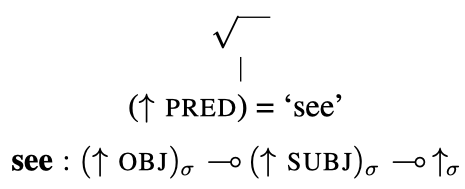
\includegraphics[scale=.3]{figures/Morphology/see-tree.png}}
}
%
The c-structure is licensed by c-structure rules of the usual kind,
but containing categories like \dmroot, which are less familiar in
LFG. Thus, the annotated c-structure rule for licensing 
\exrr{lrfg-simple-subtree} in a c-structure would be as follows, leaving the mother
category underspecified and similarly the sister of \dmroot:
%
\ea
\phraserule{X$^n$}{\csn{\dmroot}{\updown}
    \hspace*{1em} \csn{X$^{m,~m \leq n}$}{\updown}}
\z
%
\largerpage
Note that it is X$^m$ that projects the c-structure mother X$^n$ in a
co-head structure with
\dmroot. Thus, X is necessarily a functional category
\citep[ch.\,6]{BresnanEtAl2016}. 

In short, we can think of the lefthand side of a Vocabulary Item as a
tree admissibility condition \citep{mcca:68} on a subtree whose 
preterminal yield is the list of categories in the first coordinate of
the $\nu$ function such that the f-description in the second
coordinate and the meaning constructors in the third are the union of
its terminal yield. Alternatively, we can think of it in terms of
terminal expansions, such as:
%
\eabox{
\phraserule{\dmroot}{%
    \ensuremath{\left\{
    \begin{array}[c]{@{}l@{}}
      \aset{(\UP~\PRED) = \predvall{see},
      \formula{\cons{see}:(\UP~\OBJ)\sig \linimp (\UP~\SUBJ)\sig \linimp \upsigb}},\\\multicolumn{1}{c}{\vdots}
    \end{array}
  \right\}
}
}
}
  %
  \largerpage
  We prefer the tree admissibility route, but observe that whether we
  go that route or the terminal expansion route, there is no
  information about form in the input side of the Vocabulary
  Item. That is the job of the $\nu$ correspondence function. Recall
  that $\nu$ maps the information in c-structure terminals and
  c-structure categorial information to v-structures, as shown in
  (\ref{ex:waab-vi}--\ref{ex:see-vi}).


Here is an example from Ojibwe (\textit{Anishinaabemowin},
Algonquian; \citealt[288]{Melchin2020}):
%
\ea\label{ex:ojibwe-see} Ojibwe\\
  \gll
  gi- gii- waab -am -igw -naan -ag \\
    2 \feat{pst} see \feat{vta} \feat{inv} 1\feat{pl} 3\feat{pl}\\
  \glt `They saw us(incl).'
\z
%
The \lrfg\ c-structure and f-structure and the
$\nu$ correspondence from c-structure to v-structure
are shown in \figref{fig:objiwe-cs-fs-vs} \citep[288]{Melchin2020}.
%
%
Note that we have only shown the form part of each v-structure, and
only using an orthographic rather than phonemic
representation. V-structures also minimally contain prosodic
information --- such as information about phonological dependency
(e.g., for \aterm{clisis}) and the identity of the host (e.g., for
\aterm{affixation}) --- and any {purely} morphological information
(e.g., \aterm{inflectional class}).
\citet{asudeh;bogel;siddiqi-momot} propose the v-structure
representation that is schematized in \exrr{vs}. % See
% \citet{asudeh;siddiqi-lfg22} for some further discussion.
%
\eabox{\label{ex:vs}
  \avm[style=fstr]{
    [\begin{tabular}{@{}l@{}}!phon(ological)! \\
    !rep(resentation)! \vspace*{.5ex}
     \end{tabular}
     & \textup{\textit{phonological
      realization \& conditions}}\\
     !p(rosodic)frame! \vspace*{.5ex}& \textup{\textit{prosodic unit}}\\
     !p(rosodic)level! \vspace*{.5ex}& 1|2\\
     !dep(endence)! \vspace*{1.5ex} & \{left,right\}\\
     class \vspace*{.5ex} & \{\textup{\textit{inflectional classes}}\}\\
     type \vspace*{1.5ex} & verbal|nominal|adjectival\\
     host & [identity & aunt|niece\\
       \{ [phon.rep \hspace*{1.5em} & \ldots\\
           pframe & \ldots\ \\
           plevel & \ldots\\
           class & \ldots\\
           type & \ldots] \}       
       ]
    ]
}
}
  

\begin{sidewaysfigure}
  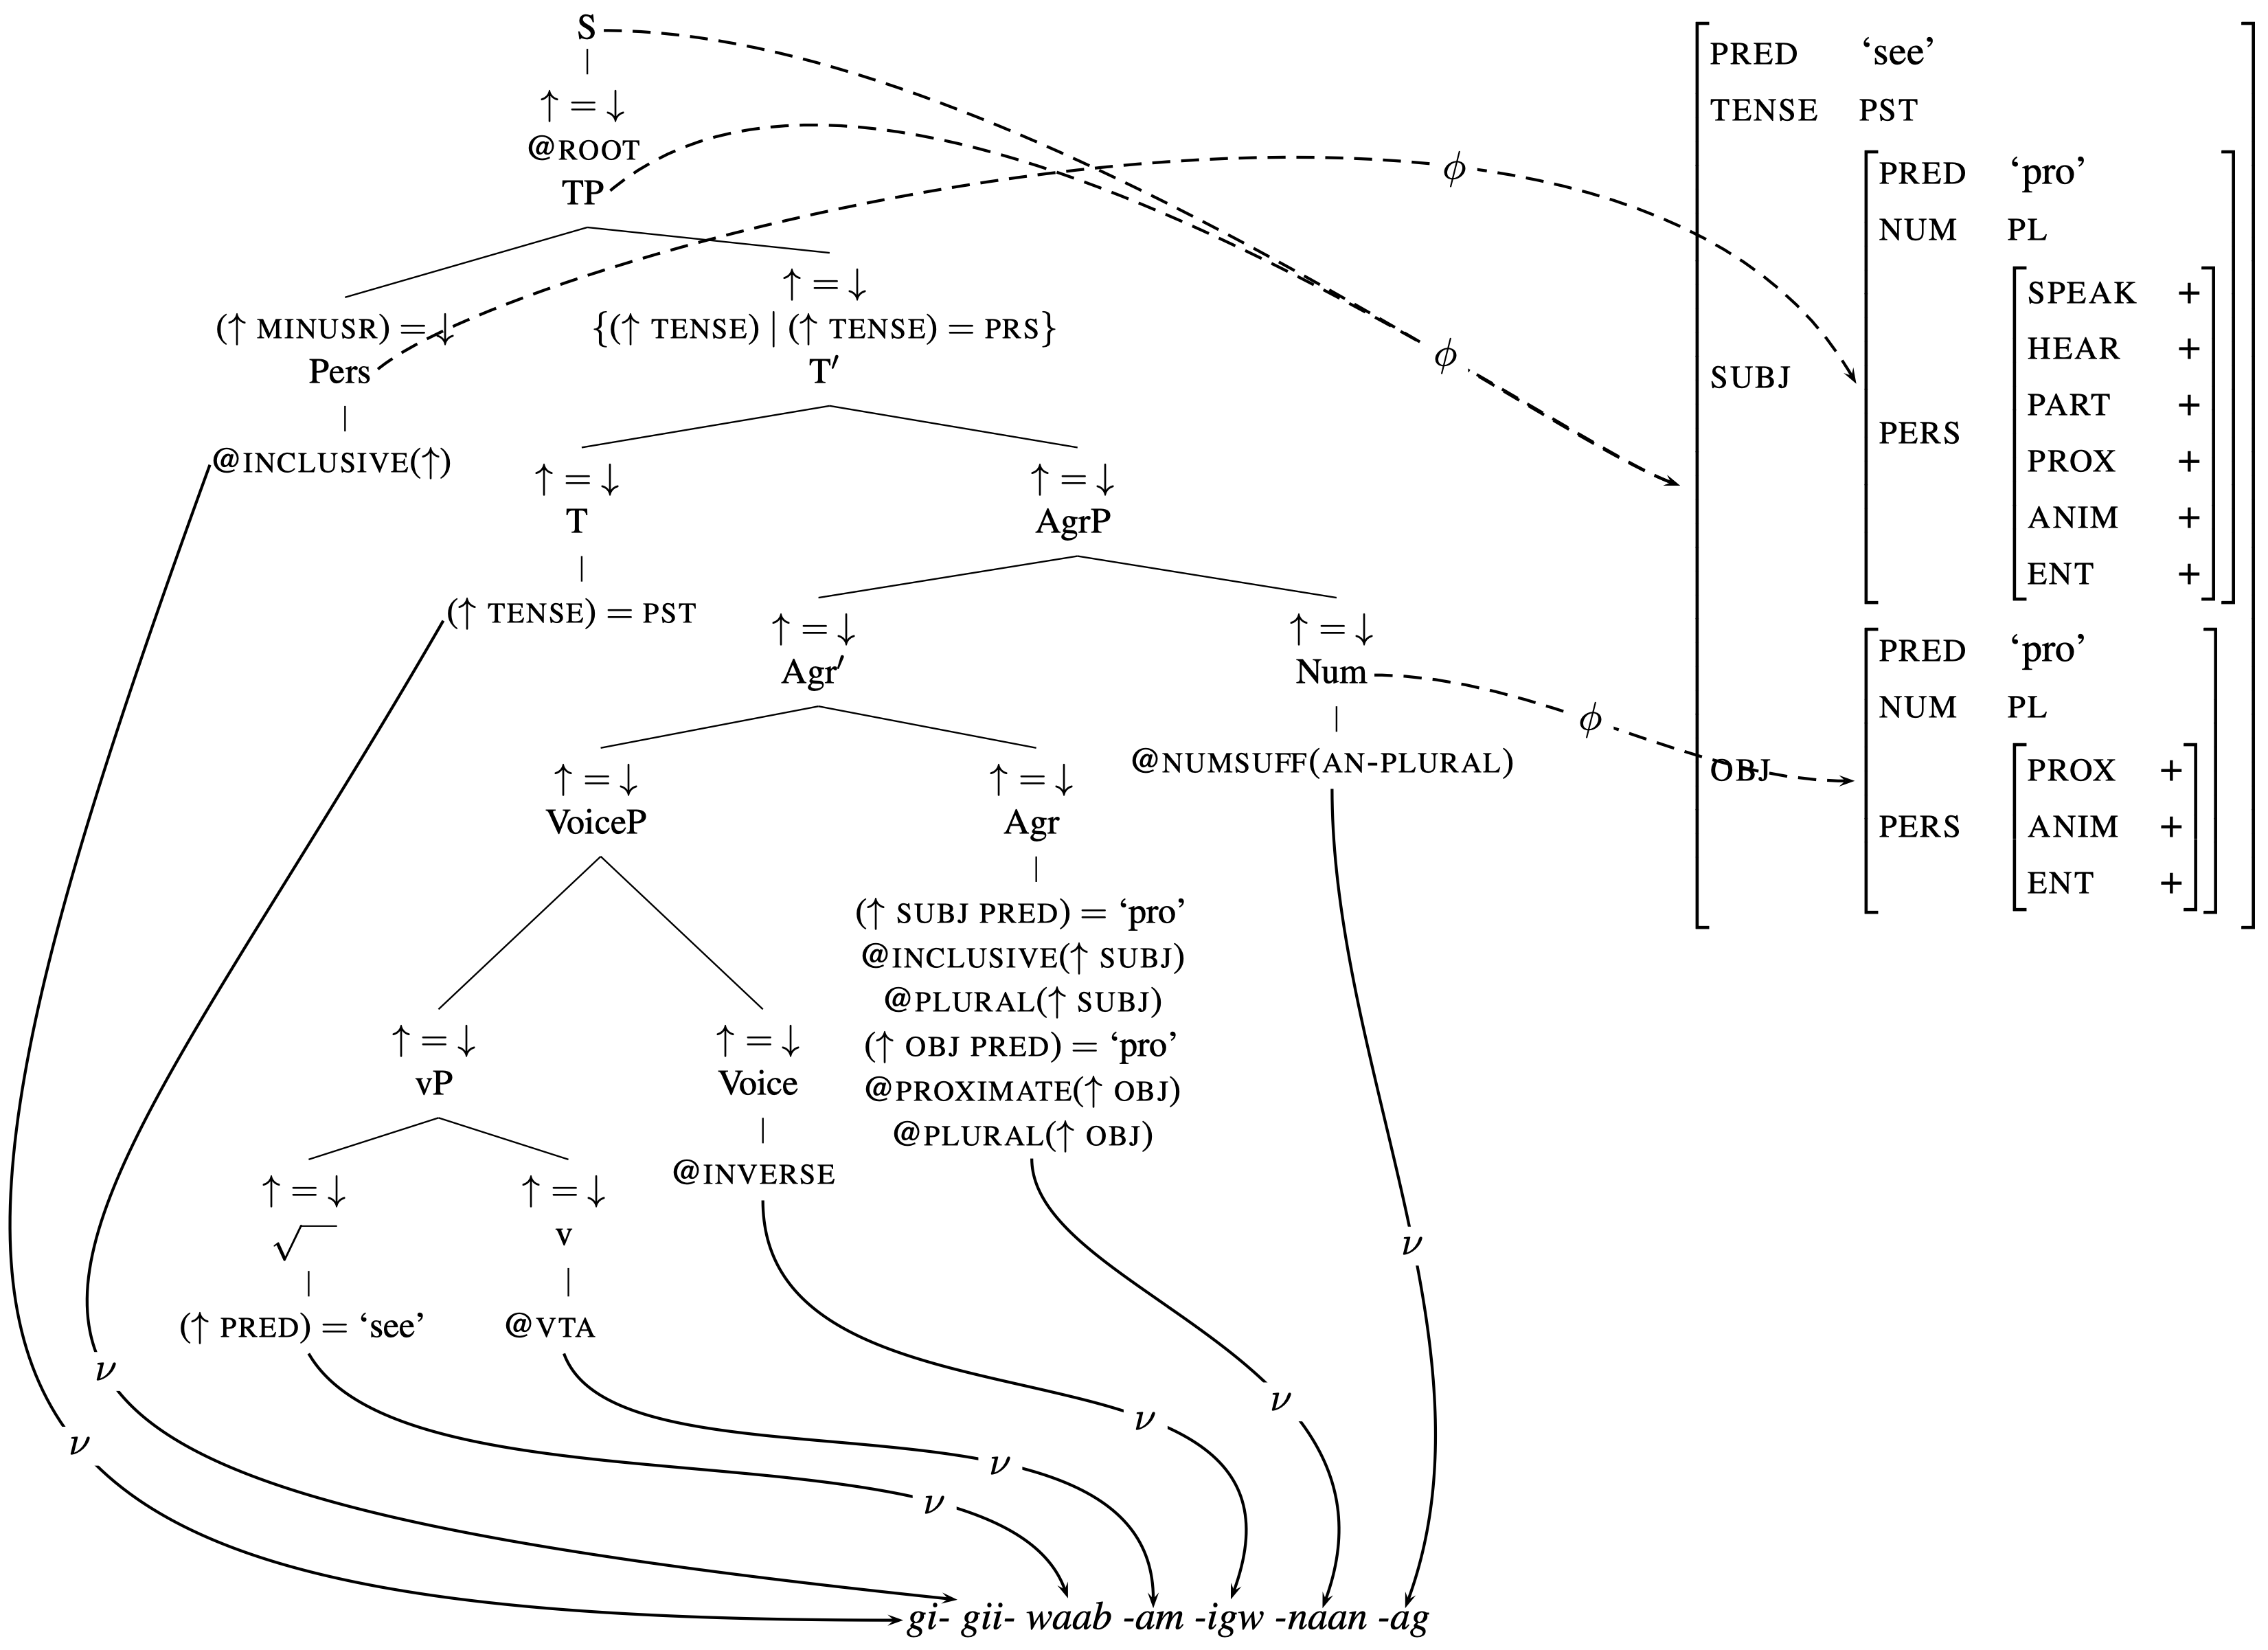
\includegraphics[width=\textwidth]{figures/Morphology/ojibwe-cs-fs-vs.png}
  \caption{\lrfg\ c-structure, f-structure, and (simplified)
    v-structure for Ojibwe \aword{gigiiwaabamigwnaanag} \attrns{They
      saw us(incl)}}
  \label{fig:objiwe-cs-fs-vs}
\end{sidewaysfigure}
\clearpage


  %\attop{
%     \avm{%
%       [phon\(ological\)rep\(resentation\) & \aterm{phonological
%         realization \& conditions}\\
%       p\(rosodic\)frame & \textit{prosodic unit}\\
%       p\(rosodic\)level & 1|2\\
%       dep\(endence\) & & lt|rt\\
%       class & \{\aterm{inflectional classes}\}\\
%       type & verbal|% 
%                    nominal|adjectival\\
%       host &    \sqz{\aterm{v-structure}}
%              \avm{%
%                    [identity & aunt|niece\\
%                    phon.rep &
%                   \ldots\\
%                   pframe & \ldots\\
%                   plevel & \ldots\\
%                   class & \ldots\\
%                   type & \ldots]
%                 }
%                 ]
%               }
% }
% \z
%
A v-structure is thus a feature structure that minimally contains information
about form and morphophonology (\feat{phon.rep}, \feat{pframe},
\feat{plevel}, and \feat{dep}), properly morphological information
(\feat{class}, \feat{type}), and morphosyntactic information about its
\feat{host}, where relevant. All features can be left underspecified
(i.e., when they are not mentioned in the description that defines the
v-structure). 

The obvious point of contrast between \lrfg\ and LFG concerns
the Lexicalist Hypothesis \citep{chomsky1970remarks,lapointe80}:  
%
\ea
\aterm{Lexicalist Hypothesis}\\
  No syntactic rule can refer to elements of morphological
  structure. \hfill \citep[8]{lapointe80}
\z
%
In LFG, this is captured in the \aterm{Lexical Integrity
    Principle}, through formulations like the following:
%
\ea \label{ex:lip} \aterm{Lexical Integrity}\\
    Morphologically complete words are leaves of the c-structure tree,
    and each leaf corresponds to one and only one c-structure
    node.\label{lipa} \\ \mbox{\citep[92]{BresnanEtAl2016}}
  \z
  %
  This statement has two parts:
  \begin{enumerate}
  \item \label{item:morphology:1} \lrfg\ \emph{upholds} the part that states that ``each leaf
    corresponds to one and only one c-structure node''.

  \item \label{item:morphology:2} \lrfg\ \emph{rejects} the part that states that
    ``morphologically complete words are leaves of the c-structure
    tree''.
  \end{enumerate}
  Clearly, the c-structure leaves/terminals in \lrfg\ are not
  ``morphologically complete words''. The c-structure leaves/terminals
  are feature bundles that \emph{map} to form, but the form itself is
  not part of the terminal node; hence \ref{item:morphology:2}. Yet there is never multidominance in
  an \lrfg\ c-structure; hence \ref{item:morphology:1}.

  However, notice that the notion \aterm{morphologically complete word}
  is left unanalyzed in the definition in \exrr{lip}.  In fact, it is
  far from clear that ``morphologically complete word'' is a coherent
  notion \citep[for discussion, see e.g.,][]{anderson82-wm}. The essential
  problem is that there are multiple relevant notions of wordhood, and
  they don't align on a single type of object that we can point to and
  unambiguously and confidently call a word
  \citep{disciullo:word}.\footnote{This is a long and broad
    discussion that we cannot possibly do justice to here.} In fact,
  there can be mismatches between the phonological, syntactic, and
  semantic aspects of words \citep{marantz1997no}. Of course, the LFG
  Correspondence Architecture is designed around the notion of
  mismatches between modules, which is carried over into \lrfg. 


  %%%%% XX old section was here %%%%
  

\subsubsection{Conditions on exponence}
\label{sec:Morph:conditions-exponence}  

Recall that the exponence  function ($\expone$) maps a triple
to a v-structure. The first argument of the triple is a
list of preterminal categories, typically of length 1, which are taken
in the linear order they appear in the tree.  The second argument is
itself a function, \fsfunc, which maps an f-description to the set of
f-structures that satisfy the description; i.e.\
$\Phi(d \in D) = \{f \in F\ |\ f \models d\}$, where $D$ is the set of
valid f-descriptions and $F$ is the set of f-structures.\footnote{We
  thank Ron Kaplan (p.c.) for discussion of this point. Any remaining
  errors are our own.}  The third argument is a set that includes
\aterm{meaning constructors} from Glue Semantics
\citep[Glue;][]{Dalrymple:Glue,dalrymple01,DLM:LFG,Asudeh12,asudeh22}.

Let $V^i$ be the domain of the exponence function $\nu$ in some
language $L$, i.e.\ the set of inputs to Vocabulary Items in $L$. We
write $V^i(\alpha)$ to indicate the domain of some particular
Vocabulary Item, $\alpha$. We write $\pi_n(V^i(\alpha))$ to indicate
the $n${th} projection of $V^i(\alpha)$. For example,
$\pi_1(V^i(\alpha))$ returns the c-structure list in the first
projection of the input to Vocabulary Item $\alpha$.\footnote{This
  $\pi$ is just standard notation for retrieving arguments to
  functions and should not be mistaken for a correspondence function.}
The following
conditions on exponence hold based on the input side of the $\nu$
correspondence function
\citep{asudeh;siddiqi-lfg22}.\footnote{Note that all these conditions
  are Paninian, as is typical in morphological analysis. The analog in
PFM is actually called Panini's Principle \citep{Stu01} and in DM it
is called the
Subset Principle \citep{hallemarantz}.}
%
\ea
  \begin{sloppypar}
    \amic[$(\alpha,\beta)$]  returns whichever of $\alpha$,$\beta$ has
  the longest list of overlapping c-structure
  categories.%
  \end{sloppypar}

  \emph{Intuition.} Prefer portmanteau forms, 
    whenever possible, on c-structural grounds.  Choose the VI that realizes the greater list of categories. \\[1ex]
    \emph{Formalization.} We define a function \cons{span} that 
    compares two lists for overlap.\footnote{\label{fn:span}
      \citet{asudeh;siddiqi-lfg22} define \cons{span} as follows:

      \noindent
      \formula{\cons{span}(\aterm{list}_1,\aterm{list}_2)} $=$ \(
      \begin{cases}
        \formula{
          \textsf{first}(\aterm{list}_1) =
          \textsf{first}(\aterm{list}_2) \wedge\
          \cons{span}(\textsf{rest}(\aterm{list}_1),\textsf{rest}(\aterm{list}_2))
        } 
        \\
        \formula{
          \aterm{list}_1 \neq \aterm{elist}\
          \wedge\ \aterm{list}_2 = \aterm{elist}
        } 
      \end{cases}
      \)
      }

 Given two Vocabulary Items, $\alpha$ and $\beta$,\\
    \scalebox{0.875}{\amic[($\alpha,\beta$)] $=$
    \(
        \begin{cases}
          \alpha\ \mathbf{if}\ 
          \pi_1(V^i(\alpha)) = f 
          \wedge\ \pi_1 (V^i(\beta)) = g\ \wedge\ \cons{span}(f,g)
          \\
          \beta \ \mathbf{if}\ 
          \pi_1(V^i(\alpha)) = f 
          \wedge\ \pi_1(V^i(\beta)) = g\ \wedge\ \cons{span}(g,f)
          \\
          \bot\ \mathbf{otherwise}
        \end{cases}
        \)}
    \z
    
    \ea
    \amif[$(\alpha,\beta)$] returns whichever of $\alpha$,$\beta$ has
  the most specific f-structure in the set of f-structures returned by
  $\Phi$ applied to $\alpha/\beta$'s
  collected f-description. \\[1ex]
  \emph{Intuition.} Prefer portmanteau forms, 
    whenever possible, on f-structural grounds. Choose the VI that defines
    an f-structure that contains the great\-er set of features.\\[1ex]
  \emph{Formalization.} The proper subsumption relation on
  f-structures \citep[ch.~5]{BresnanEtAl2016} is used to capture the
  intuition.

Given two VIs, $\alpha$ and $\beta$, \\ \amif[$(\alpha,\beta)$] $=$
        \scalebox{0.825}{\(
        \begin{cases}
          \alpha\ \mathbf{if}\ \exists f\forall g.f \in
          \pi_2(V^i(\alpha))
          \wedge g \in \pi_2(V^i(\beta)) \wedge g \sqsubset f \\
          \beta \ \mathbf{if}\ \exists f\forall g.f \in
          \pi_2(V^i(\beta))
          \wedge g \in \pi_2(V^i(\alpha)) \wedge g \sqsubset f \\
          \bot\ \mathbf{otherwise}
        \end{cases}
        \)}
\z


\ea
  \begin{sloppypar}
    \noindent
    \amis[$(\alpha,\beta)$] returns whichever Vocabulary Item has the
    more specific meaning.
  \end{sloppypar}
%\\[1ex]
  \begin{sloppypar}
    \emph{Intuition.} Prefer portmanteau forms, wherever possible, on
    semantic grounds. Choose the VI whose denotation is more
    semantically contentful.
  \end{sloppypar}
%\\[1ex]
  \emph{Formalization.} The proper subset relation on set-denoting expressions  is
  used to capture the intuition.

 \begin{tabular}[t]{@{}l} 
    Given two Vocabulary Items, $\alpha$ and $\beta$,\\
    \scalebox{.825}{\amis[($\alpha,\beta$)] $=$
    \(
    \begin{cases}
      \alpha\ \mathbf{if}\ f = \pi_3(V^i(\alpha)) \wedge g =
      \pi_3(V^i(\beta)) \wedge \sem{$f$} \subset \sem{\raisebox{0.25ex}{$g$}}\\
      \beta\ \mathbf{if}\ f = \pi_3(V^i(\alpha)) \wedge g =
      \pi_3(V^i(\beta)) \wedge \sem{\raisebox{0.25ex}{$g$}} \subset \sem{$f$}\\
      \bot\ \mathbf{otherwise}
    \end{cases}
    \)}
 \end{tabular}
 
\z
%
In addition, there is a constraint on exponence that concerns the
output of the $\nu$ correspondence function
\citep{asudeh;siddiqi-lfg22}, i.e. the expression of prosodic and
phonological information. Let $V^o$
  be the co-domain of the exponence function $\nu$ in some language
  $L$, i.e.\ the set of outputs of Vocabulary Items in $L$. We write
  $V^o(\alpha)$ to indicate the co-domain of some particular
  Vocabulary Item, $\alpha$ (i.e., the output vocabulary structure).
%
  \ea \label{ex:msp} \amsp[$(\alpha,\beta)$] returns whichever Vocabulary Item has the
  most restrictions on its phonological context.
  \\[1ex]
  \emph{Intuition.} Prefer affixes whenever possible.
  \\[1ex]
  \emph{Formalization.} The proper subsumption relation on feature
  structures --- i.e., v-structures --- is used to capture the
  intuition.
  
  \begin{tabular}[t]{@{}l} 
    Given two Vocabulary Items, $\alpha$ and $\beta$,\\ \amsp[($\alpha,\beta$)] $=$
    \(
    \begin{cases}
      \alpha\ \mathbf{if}\ (V^o(\beta)\ \feat{host}) \sqsubset (V^o(\alpha)\ \feat{host})\\
      \beta\ \mathbf{if}\ (V^o(\alpha)\ \feat{host}) \sqsubset (V^o(\beta)\ \feat{host})\\
      \bot\ \mathbf{otherwise}
    \end{cases}
    \)
  \end{tabular} 
\z
%
The upshot is that \amsp[] chooses the VI whose
output v-structure has more specific content in the \feat{host}
feature.\footnote{Note that if ($f$ \feat{feat}) does not exist, ($f$
  \feat{feat}) resolves to the empty feature structure, notated
  $\bot$ 
  (not to be confused with the $\bot$ explicitly mentioned in the
  constraints above). as it's the bottom of the f-structure lattice. The empty f-structure subsumes all
  f-structures. Therefore, if ($v$
  \feat{host}) does not exist, but  ($v'$ \feat{host}) does exist, then
  ($v$ \feat{host}) $\sqsubset$ ($v'$ \feat{host}) returns true. If
  ($v'$ \feat{host}) also does not exist, then ($v$ \feat{host})
  $\sqsubset$ ($v'$ \feat{host}) returns false, since it is false that
  $\bot$ \emph{properly} subsumes $\bot$.}   

% We have used a new relation based on standard subsumption,
% \pathsubsume, in \exrr{msp}. We can call this relation
% \aterm{relativized subsumption} or \aterm{path subsumption}. The
% relation is necessary in order to handle the case of comparing
% structures that are relativized according to some feature/path, in
% this case \feat{host}. In other words, if $\alpha$ does not have a
% \feat{host} feature but $\beta$ does, we want
% $\alpha \pathsubsume \beta$ to be true, whereas
% $\alpha \sqsubset \beta$ would be false. We define \pathsubsume\ as
% follows:

% \begin{examples}
% \item \label{ex:pathsub}
%   Given an f-structure $f$, an f-structure $g$, and paths $\alpha$ and $\beta$:\\
%   \ensuremath{(f~\alpha) \pathsubsume (g~\beta)} is true iff
%   \(
%   \begin{cases}
%     (f~\alpha) \sqsubset (g~\beta); or\\
%     \neg (f~\alpha) \wedge (g~\beta)
%     \end{cases}
%     \) 
% \end{examples}
% %
% \begin{sloppypar}
%   \noindent
%   We have presented the definition by cases, but equivalently we could
%   write \ensuremath{[(f~\alpha) \pathsubsume (g~\beta)] \leftrightarrow
%     [(f~\alpha) \sqsubset (g~\beta) \vee [\neg (f~\alpha) \wedge (g~\beta)]]}.
% \end{sloppypar}

Note that \amic[] and \amif[] are \emph{morphosyntactic}
constraints, \amis[] is a \emph{morphosemantic} constraint, and
\amsp[] is a \emph{morphophonological} constraint.  Note also
that each constraint can result in a tie, represented by
$\bot$. However, there are regularities in the mappings/interfaces
between structures, so it would be unlikely for all four 
constraints to yield $\bot$. We are not currently aware of any
empirical case that would merit such an analysis. Lastly, it is
important to note that these constraints apply simultaneously and
universally (whenever they can), much like standard constraints and
equations in LFG. There is no constraint-ordering and the constraints
are not soft constraints.\footnote{An anonymous reviewer wonders what the
  system would do if one constraint picks $\alpha$ and another picks
  $\beta$. This is an interesting point that deserves further
  investigation and we thank the reviewer for highlighting it.}


In sum, \lrfg\ is a daughter framework of LFG that uses the LFG
formalism in a conservative fashion. However, \lrfg\ theory makes some
different assumptions from traditional LFG theory. Namely, it
rearranges the Correspondence Architecture, adds a new structure with
new properties (v-structure), upholds only part of the Lexical
Integrity Principle, and has a more articulated c-structure than
standard LFG, in order to provide a morphemic theory of
morphology. These theoretical distinctions are due to the influence of
DM, since \lrfg\ is also a daughter framework of DM.

\begin{sloppypar}
  As its name states, Lexical-Realizational Functional Grammar is a
  \aterm{lexical-realizational} theory of morphology. It is
  \aterm{morphemic}, \aterm{Item-and-Arrangement}, and
  \aterm{morphosyntactic}.
  %(i.e., gives up part of Lexical Integrity).
\end{sloppypar}

\section{Conclusion}
A feature of LFG is its f-descriptions, which can occur in both
lexical entries and on c-structure nodes. The result is that both
morphology and syntax can contribute information to f-structure. This
\ascare{common language} between morphology and syntax has allowed
LFG to remain agnostic about the precise nature of morphology. In its
initial construal as just a theory of syntax, based around c-structure
and f-structure, this was pretty harmless. But once a general
grammatical architecture, the Correspondence Architecture, was
proposed \citep{kapl:89,kaplan1995formal}, LFG began to owe a better account of how it
interfaces with morphology. 

In early LFG, morphology was generally done incrementally, using
annotated phrase structure rules of the same kind that license
c-structures, but whose categories are morphological instead of
syntactic. Morphological theory in general, though, has been
converging on the idea that morphology is realizational, not
incremental. Therefore, more recent work has focused on exploring the
syntax--morphology interface
\citep[ch.\,12]{dalrymple15,DLM:LFG} in light of an interface with
realizational morphology. This work can be thought of as
providing a universal adapter between LFG syntax and some kind of
realizational morphology. Much of the theoretical work on
morphology for LFG over the last couple of decades has focused on
interfacing LFG with Paradigm Function Morphology. Other recent work has
presented an alternative in the guise of \lrfg, a framework that instead
interfaces LFG with Distributed Morphology.
 
The existence of two different approaches to morphological realization
in LFG, i.e.\ PFM and \lrfg, mirrors two different interpretations of
\ascare{morphological complexity} as a set of phenomena requiring
explanation. \aterm{Paradigmatic} morphological complexity
\citep[see, e.g.,][]{baerman;etal2017} concerns
complex patterns of syncretism, root allomorphy, and templatic
morphology. \aterm{Syntagmatic}  morphological complexity 
concerns concatenative morphology whose structures seem to encode
syntactic structure, in other words structure \emph{within} what we
pretheoretically call words. PFM addresses the former kind of
morphological complexity, while \lrfg\ addresses the latter. 

\section*{Acknowledgements}

We thank Farrell Ackerman, Jim Blevins, Greg Stump, and Andy Spencer
for fruitful discussions about some of the issues covered here over
the last several years. Greg in particular deserves a special thank
you for reading some precursors of this material, especially
\sectref{sec:Morph:morph-theory}. We also thank our students$^\dag$ and
collaborators$^\ddag$ on the \lrfg\ project: Oleg Belyaev$^\ddag$,
Bronwyn Bjorkman$^\ddag$, Tina B\"{o}gel$^\ddag$, Veronica
Burrage$^\dag$, Michael Everdell$^\ddag$, Paul B. Melchin$^\ddag$,
Will Oxford$^\ddag$, and Sam Turnbull$^\dag$. Thank you to the
anonymous reviewers of this paper for helping us to improve it,
including spotting some serious errors. Last
but most definitely not least, we thank Mary Dalrymple for taking on
the mammoth task of editing this volume, for her patience and help
with this particular paper, and for the inspiration that her own work
on morphology in LFG has provided us. All remaining errors and
misconceptions are our own.

\section*{Abbreviations}

Besides the abbreviations from the Leipzig Glossing Conventions, this
chapter uses the following abbreviations.\medskip

\noindent\begin{tabularx}{.45\textwidth}{lQ}
\gloss{inv} & inverse voice \\
\gloss{prop} & proprietive case \\
\end{tabularx}\begin{tabularx}{.5\textwidth}{lQ}
\gloss{vta} & verb transitive animate object \\
\\
\end{tabularx}

  
\sloppy
\printbibliography[heading=subbibliography,notkeyword=this]
\end{document}
